\section{SLR-Parser}
In diesem Abschnitt zeigen wir, wie wir f\"ur eine gegebene kontextfreie Grammatik $G$ 
die im letzten Abschnitt verwendeten Funktionen 
\\[0.2cm]
\hspace*{1.3cm}
$\textsl{action}: Q \times T \rightarrow \textsl{Action}$ \quad and \quad $\textsl{goto}: Q \times V \rightarrow Q$
\\[0.2cm]
berechnen k\"onnen.  Dazu kl\"aren wir als erstes, welche Informationen die in der Menge $Q$ enthaltenen Zust\"ande 
enthalten sollen.  Wir werden diese Zust\"ande so definieren, dass sie die Information enthalten,
welche Regel der Shift-Reduce-Parser anzuwenden versucht, welcher Teil der rechten Seite einer Grammatik-Regel 
bereits erkannt worden ist und was noch erwartet wird.  Zu diesem Zweck definieren wir den Begriff
einer \emph{markierten Regel}.   In der englischen Originalliteratur \cite{knuth:65} wird hier
ungl\"ucklicherweise der inhaltsleere Begriff ``\emph{item}'' verwendet.

\begin{Definition}[markierte Regel]
  Eine \emph{markierte Regel} einer Grammatik $G = \langle V, T, R, s \rangle$ ist ein Tripel
  \\[0.2cm]
  \hspace*{1.3cm}
  $\langle a, \beta, \gamma \rangle$,
  \\[0.2cm]
  f\"ur das gilt
  \\[0.2cm]
  \hspace*{1.3cm}
  $(a \rightarrow \beta \gamma) \in R$.
  \\[0.2cm]
  Wir schreiben eine markierte Regel $\langle a, \beta, \gamma \rangle$ als
  \\[0.2cm]
  \hspace*{1.3cm}
  $a \rightarrow \beta \bullet \gamma$. \qed 
\end{Definition}

\noindent
Die markierte Regel $a \rightarrow \beta \bullet \gamma$ dr\"uckt aus, dass der Parser versucht,
mit der Regel $a \rightarrow \beta \gamma$ ein $a$ zu parsen, dabei schon $\beta$ gesehen
hat und als n\"achstes versucht, $\gamma$ zu erkennen.  Das Zeichen $\bullet$ markiert also die
Position innerhalb der rechten Seite der Regel, bis zu der wir die rechte Seite der Regel
schon gelesen haben.
Die Idee ist jetzt, dass wir die Zust\"ande eines SLR-Parsers als Mengen von markierten Regeln
darstellen k\"onnen.  Um diese Idee zu verschaulichen, betrachten wir ein konkretes Beispiel:
Wir gehen von der in Abbildung \ref{fig:Expr.grammar} auf Seite \pageref{fig:Expr.grammar}
gezeigten Grammatik aus, wobei wir diese Grammatik noch um ein neues Start-Symbol $\widehat{s}$
und die Regel
\\[0.2cm]
\hspace*{1.3cm} $\widehat{s} \rightarrow  \textsl{expr}\;\textsc{Eof}$
\\[0.2cm]
erweitern.  Der Start-Zustand enth\"alt offenbar die markierte Regel
\\[0.2cm]
\hspace*{1.3cm} $\widehat{s} \rightarrow \varepsilon \bullet \textsl{expr}\, \textsc{Eof}$,
\\[0.2cm]
denn am Anfang versuchen wir ja, das Start-Symbol $\widehat{s}$ herzuleiten.  Die Komponente
$\varepsilon$ dr\"uckt aus, dass wir bisher noch nichts verarbeitet haben.  Neben dieser
markierten Regel muss der Start-Zustand dann au{\ss}erdem die markierten Regeln
\begin{enumerate}
\item $\textsl{expr} \rightarrow \varepsilon \bullet \textsl{expr} \quoted{+} \textsl{product}$,
\item $\textsl{expr} \rightarrow \varepsilon \bullet \textsl{expr} \quoted{-} \textsl{product}$
      \qquad und
\item $\textsl{expr} \rightarrow \varepsilon \bullet \textsl{product}$
\end{enumerate}
enthalten, denn es k\"onnte ja beispielsweise sein, dass wir die Regel
\\[0.2cm]
\hspace*{1.3cm}
$\textsl{expr} \rightarrow \textsl{expr} \quoted{+} \textsl{product}$
\\[0.2cm]  
verwenden m\"ussen, um die gesuchte \textsl{expr} herzuleiten.  Genauso gut k\"onnte es nat\"urlich sein,
dass wir statt dessen die Regel
\\[0.2cm]
\hspace*{1.3cm}
$\textsl{expr} \rightarrow \textsl{product}$
\\[0.2cm]
benutzen m\"ussen.  Das erkl\"art, warum wir die markierte Regel
\\[0.2cm]
\hspace*{1.3cm}
 $\textsl{expr} \rightarrow \varepsilon \bullet \textsl{product}$
\\[0.2cm]
in den Start-Zustand aufnehmen m\"ussen, denn 
da wir am Anfang noch gar nicht wissen k\"onnen, welche Regel wir ben\"otigen, muss
der Start-Zustand daher alle diese Regeln enthalten.  Haben wir erst die markierte Regel
\\[0.2cm]
\hspace*{1.3cm}
 $\textsl{expr} \rightarrow \varepsilon \bullet \textsl{product}$ 
\\[0.2cm]
zum Start-Zustand hinzugef\"ugt, so sehen wir, dass wir eventuell als n\"achstes ein $\textsl{product}$
lesen m\"ussen.  Daher sehen wir,  dass der Start-Zustand au{\ss}erdem noch die folgenden markierten
Regeln enth\"alt:  
\begin{enumerate}
\item[4.] $\textsl{product} \rightarrow \bullet\; \textsl{product} \quoted{*} \textsl{factor}$,
\item[5.] $\textsl{product} \rightarrow \bullet\; \textsl{product} \quoted{/} \textsl{factor}$,
\item[6.] $\textsl{product} \rightarrow \bullet\; \textsl{factor}$,

          Nun zeigt die sechste Regel, dass wir eventuell als erstes einen \textsl{factor}
          lesen werden.  Daher f\"ugen wir zu dem Start-Zustand auch die folgenden beiden markierten
          Regeln hinzu: 
\item[7.] $\textsl{factor} \rightarrow \bullet \quoted{(} \textsl{expr} \quoted{)}$,
\item[8.] $\textsl{factor} \rightarrow \bullet\; \textsc{Number}$.
\end{enumerate}
Insgesamt sehen wir, dass der Start-Zustand aus einer Menge mit 8 markierten Regeln besteht.
Das oben gezeigte System, aus einer gegebenen Regel weitere Regeln abzuleiten,
formalisieren wir in dem Begriff des \emph{Abschlusses} einer Menge von markierten
Regeln.

\begin{Definition}[$\textsl{closure}(\mathcal{M})$]
  Es sei $\mathcal{M}$ eine Menge markierter Regeln.  Dann definieren wir den \emph{Abschluss} dieser Menge
  als die kleinste Menge $\mathcal{K}$ markierter Regeln, f\"ur die folgendes gilt:
  \begin{enumerate}
  \item $\mathcal{M} \subseteq \mathcal{K}$,

        der Abschluss umfasst also die urspr\"ungliche Regel-Menge.
  \item Ist einerseits
        \\[0.2cm]
        \hspace*{1.3cm}
        $a \rightarrow \beta \bullet c\, \delta$
        \\[0.2cm]
        eine markierte Regel aus der Menge $\mathcal{K}$, wobei $c$ eine syntaktische
        Variable ist, und ist andererseits
        \\[0.2cm]
        \hspace*{1.3cm}
        $c \rightarrow \gamma$
        \\[0.2cm]
        eine Grammatik-Regel der zu Grunde liegenden Grammatik $G$, so ist auch die markierte
        Regel 
        \\[0.2cm]
        \hspace*{1.3cm}
        $c \rightarrow \bullet \gamma$
        \\[0.2cm]
        ein Element der Menge $\mathcal{K}$.  Als Formel schreibt sich dies wie folgt:
        \\[0.2cm]
        \hspace*{1.3cm}
        $(a \rightarrow \beta \bullet c\, \delta) \in \mathcal{K} 
         \;\wedge\; 
         (c \rightarrow \gamma) \in R
         \;\Rightarrow\; (c \rightarrow \bullet \gamma) \in \mathcal{K}
        $
  \end{enumerate}
  Die so definierte Menge $\mathcal{K}$ ist eindeutig bestimmt und wird im Folgenden mit
  $\textsl{closure}(\mathcal{M})$ bezeichnet. \qed
\end{Definition}

\noindent
\textbf{Bemerkung}: Wenn Sie sich an den Earley-Algorithmus erinnern, dann sehen Sie, dass bei der
Berechnung des Abschlusses dieselbe Berechnung wie bei der Vorhersage-Operation
des  Earley-Algorithmus durchgef\"uhrt wird.  \eox
\vspace*{0.3cm}

\noindent
F\"ur eine gegebene Menge $\mathcal{M}$ von markierten Regeln, kann die Berechnung von
$\mathcal{K} := \textsl{closure}(\mathcal{M})$ iterativ erfolgen:
\begin{enumerate}
\item Zun\"achst setzen wir $\mathcal{K} := \mathcal{M}$.
\item Anschlie{\ss}end suchen wir alle Regeln der Form
      \\[0.2cm]
      \hspace*{1.3cm}
      $a \rightarrow \beta \bullet c\, \delta$
      \\[0.2cm]
      aus der Menge $\mathcal{K}$, f\"ur die $c$ eine syntaktische Variable ist und f\"ugen dann
      f\"ur alle Regeln der Form $c \rightarrow \gamma$ die neue markierte Regel
      \\[0.2cm]
      \hspace*{1.3cm}
      $c \rightarrow \bullet\gamma$
      \\[0.2cm]
      in die Menge $\mathcal{K}$ ein.

      Dieser Schritt wird solange iteriert, bis keine neuen Regeln mehr gefunden werden.
\end{enumerate}
\pagebreak

\example
Wir gehen von der in Abbildung
\ref{fig:Expr.grammar} auf Seite \pageref{fig:Expr.grammar} gezeigten Grammatik aus und betrachten
die Menge
\[ \mathcal{M} := 
   \bigl\{ \textsl{product} \rightarrow \textsl{product} \quoted{*}\! \bullet \textsl{factor} \bigr\}
\]
F\"ur die Menge $\textsl{closure}(\mathcal{M})$ finden wir dann
\\[0.2cm]
\hspace*{1.3cm}
$ 
\begin{array}[b]{lcll}
\textsl{closure}(\mathcal{M}) 
 & = & \bigl\{ &
         \textsl{product} \rightarrow \textsl{product} \quoted{*}\! \bullet \textsl{factor}, \\
   & & & \textsl{factor}  \rightarrow \bullet \quoted{(} \textsl{expr} \quoted{)}\!\!,          \\
   & & & \textsl{factor}  \rightarrow \bullet \;\textsc{Number}                                  \\
   & & \bigr\}. & \hspace*{8cm} 
\end{array}$  \eox
\vspace*{0.3cm}


\noindent
Unser Ziel ist es, f\"ur eine gegebene kontextfreie Grammatik $G = \langle V, T, R, s \rangle$ einen
Shift-Reduce-Parser 
\\[0.2cm]
\hspace*{1.3cm}
$P = \langle Q, q_0, \textsl{action}, \textsl{goto} \rangle$
\\[0.2cm]
zu definieren.  Um dieses Ziel zu erreichen, m\"ussen wir uns als erstes \"uberlegen,
wie wir die Menge $Q$ der Zust\"ande definieren wollen, denn dann funktioniert die Definition der
restlichen Komponenten fast von alleine.  Die Idee ist, dass wir die Zust\"ande
als Mengen von markierten Regeln definieren.
Wir definieren zun\"achst
\\[0.2cm]
\hspace*{1.3cm}
$\Gamma := \bigl\{ a \rightarrow \beta \bullet \gamma \mid (a \rightarrow \alpha \gamma) \in R \bigr\}$
\\[0.2cm]
als die Menge aller markierten Regeln der Grammatik.  Nun ist es allerdings nicht sinnvoll,
beliebige Teilmengen von $\Gamma$ als Zust\"ande zuzulassen:  Eine Teilmenge $\mathcal{M}
\subseteq \Gamma$ kommt nur dann als Zustand in Betracht, wenn die Menge $\mathcal{M}$ unter
der Funktion $\textsl{closure}()$ \emph{abgeschlossen} ist, wenn also
$\textsl{closure}(\mathcal{M}) = \mathcal{M}$ gilt.  Wir definieren daher
\\[0.2cm]
\hspace*{1.3cm}
$Q := \bigl\{ \mathcal{M} \in 2^\Gamma \mid \textsl{closure}(\mathcal{M}) = \mathcal{M} \bigr\}$.
\\[0.2cm]
Die Interpretation der Mengen $\mathcal{M} \in Q$ ist die, dass ein Zustand $\mathcal{M}$ genau die
markierten Grammatik-Regeln enth\"alt, die in der durch den Zustand beschriebenen Situation
angewendet werden k\"onnen.


Zur Vereinfachung der folgenden Konstruktionen erweitern wir die
Grammatik $G = \langle V, T, R, s \rangle$ durch Einf\"uhrung eines neuen Start-Symbols $\widehat{s}$
und eines neuen Tokens \textsc{Eof} zu der Grammatik 
\\[0.2cm]
\hspace*{1.3cm}
$\widehat{G} = 
 \Bigl\langle V \cup \{ \widehat{s} \}, T \cup \{\textsc{Eof}\}, R \cup \{ \widehat{s} \rightarrow s\, \textsc{Eof} \}, \widehat{s} \Bigr\rangle
$.
\\[0.2cm]
Das Token \textsc{Eof} steht dabei als Abk\"urzung f\"ur \emph{\underline{e}end \underline{o}f \underline{f}ile}.
Die Grammatik $\widehat{G}$ bezeichnen wir als die \emph{augmentierte Grammatik}.  Die Verwendung der
augmentierten Grammatik erm\"oglicht die nun folgende Definition des Start-Zustands.
Wir setzen n\"amlich:
\\[0.2cm]
\hspace*{1.3cm}
$ q_0 := \textsl{closure}\Bigl( \bigl\{ \widehat{s} \rightarrow \bullet s\,\textsc{Eof} \bigr\} \Bigr)$.
\\[0.2cm]
Als n\"achstes konstruieren wir die Funktion $\textsl{goto}()$.  Die Definition lautet:
\\[0.2cm]
\hspace*{1.3cm}
$\textsl{goto}(\mathcal{M}, c) := \textsl{closure}\Bigl( \bigl\{ 
   a \rightarrow \beta\, c \bullet \delta \mid (a \rightarrow \beta \bullet c\, \delta) \in \mathcal{M} 
   \bigr\} \Bigr)
$.
\\[0.2cm]
Um diese Definition zu verstehen, nehmen wir an, dass der Parser in einem Zustand ist, in dem er
versucht, ein $a$ mit Hilfe der Regel $a \rightarrow \beta\, c\, \delta$ zu erkennen und dass dabei bereits
der Teilstring $\beta$ erkannt wurde.  Dieser Zustand wird durch die markierte Regel
\\[0.2cm]
\hspace*{1.3cm}
$a \rightarrow \beta \bullet c\, \delta$ 
\\[0.2cm] 
beschrieben.  Wird nun ein $c$ erkannt, so kann der Parser von dem Zustand, der die 
Regel $a \rightarrow \beta \bullet c\, \delta$ enth\"alt in einen Zustand, der die Regel 
$a \rightarrow \beta\, c \bullet \delta$ 
enth\"alt, \"ubergehen.  Daher erhalten wir die oben angegebene Definition der Funktion $\textsl{goto}(\mathcal{M},c)$.
F\"ur die gleich folgende Definition der Funktion $\textsl{action}(\mathcal{M}, t)$ ist es
n\"utzlich, die Definition der Funktion $\textsl{goto}$ auf Terminale zu erweitern.  
F\"ur Terminale $t \in T$ setzen wir:
\\[0.2cm]
\hspace*{1.3cm}
$\textsl{goto}(\mathcal{M}, t) := \textsl{closure}\Bigl( \bigl\{ 
   a \rightarrow \beta\, t \bullet \delta \mid (a \rightarrow \beta \bullet t\, \delta) \in \mathcal{M} 
   \bigr\} \Bigr)
$.
\\[0.2cm]
Als Letztes spezifizieren wir, wie die Funktion $\textsl{action}(\mathcal{M},t)$ f\"ur eine Menge von
markierten Regeln $\mathcal{M}$ und ein Token $t$ berechnet wird.  
Bei der Definition von $\textsl{action}(\mathcal{M},t)$ unterscheiden wir vier F\"alle.
\pagebreak

\begin{enumerate}
\item Falls $\mathcal{M}$ eine markierte Regel der Form $a \rightarrow \beta \bullet t\, \delta$
      enth\"alt, setzen wir
      \\[0.2cm]
      \hspace*{1.3cm}
      $\textsl{action}(\mathcal{M},t) := \langle \texttt{shift}, \textsl{goto}(\mathcal{M},t) \rangle$,
      \\[0.2cm]
      denn in diesem Fall versucht der Parser ein $a$ mit Hilfe der Regel $a \rightarrow \beta\, t \delta$
      zu erkennen und hat von der rechten Seite dieser Regel bereits $\beta$ erkannt.
      Ist nun das n\"achste Token im Eingabe-String tats\"achlich das Token $t$, so kann der Parser
      dieses $t$ lesen und geht dabei von dem Zustand $a \rightarrow \beta \bullet t\, \delta$ in den Zustand 
      $a \rightarrow \beta\, t \bullet \delta$ \"uber, der von der Funktion $\textsl{goto}(\mathcal{M},t)$
      berechnet wird.  Insgesamt haben wir also
      \\[0.2cm]
      \hspace*{1.3cm}
      $\textsl{action}(\mathcal{M},t) := \langle \texttt{shift}, \textsl{goto}(\mathcal{M},t) \rangle
         \quad \mbox{falls} \quad (a \rightarrow \beta \bullet t\, \delta) \in \mathcal{M}
      $.
\item Falls $\mathcal{M}$ eine markierte Regel der Form $a \rightarrow \beta \bullet$ enth\"alt
      und wenn zus\"atzlich $t \in \textsl{Follow}(a)$ gilt, dann setzen wir
      \\[0.2cm]
      \hspace*{1.3cm}
      $\textsl{action}(\mathcal{M},t) := \langle \texttt{reduce}, a \rightarrow \beta \rangle$,
      \\[0.2cm]
      denn in diesem Fall versucht der Parser ein $a$ mit Hilfe der Regel $a \rightarrow \beta$
      zu erkennen und hat bereits $\beta$ erkannt. Ist nun das n\"achste Token im Eingabe-String das Token
      $t$ und ist dar\"uber hinaus $t$ ein Token, dass auf $a$ folgen kann, gilt also 
      $t \in \textsl{Follow}(a)$, so kann der Parser die Regel $a \rightarrow \beta$ anwenden und den
      Symbol-Stack mit dieser Regel reduzieren.  Wir haben dann
      \\[0.2cm]
      \hspace*{1.3cm}
      $\textsl{action}(\mathcal{M},t) := \langle \texttt{reduce}, a \rightarrow \beta \rangle$
      \quad falls 
      $(a \rightarrow \beta\bullet) \in \mathcal{M}$, $a \not= \widehat{s}$ 
      und $t \in \textsl{Follow}(a)$ gilt.
\item Falls $\mathcal{M}$ die markierte Regel $\widehat{s} \rightarrow s \bullet \textsc{Eof}$ enth\"alt und
      wir den zu parsenden String vollst\"andig gelesen haben, setzen wir
      \\[0.2cm]
      \hspace*{1.3cm}
      $\textsl{action}(\mathcal{M},\textsc{Eof}) := \texttt{accept}$,
      \\[0.2cm]
      denn in diesem Fall versucht der Parser, $\widehat{s}$ mit Hilfe der Regel $\widehat{s} \rightarrow s\,\textsc{Eof}$
      zu erkennen und hat also bereits $s$ erkannt. Ist nun das n\"achste Token im Eingabe-String 
      das Datei-Ende-Zeichen \textsc{Eof}, 
      so liegt der zu parsende String in der durch die Grammatik $G$ spezifizierten Sprache
      $L(G)$.  Wir haben daher
      \\[0.2cm]
      \hspace*{1.3cm}
      $\textsl{action}(\mathcal{M},\textsc{Eof}) := \texttt{accept}$,
      \quad falls $(\widehat{s} \rightarrow s\bullet\textsc{Eof}) \in \mathcal{M}$.
\item In den restlichen F\"allen setzen wir
      \\[0.2cm]
      \hspace*{1.3cm}
      $\textsl{action}(\mathcal{M},t) := \texttt{error}$.
\end{enumerate}
Zwischen den ersten beiden Regeln kann es Konflikte geben.  
Wir unterscheiden zwischen zwei Arten von Konflikten.
\begin{enumerate}
\item Ein \textsl{Shift-Reduce-Konflikt} tritt auf, wenn sowohl der erste Fall als auch der zweite Fall
      vorliegt.   In diesem Fall enth\"alt die Menge $\mathcal{M}$ also zum einen eine markierte Regel
      der Form
      \\[0.2cm]
      \hspace*{1.3cm}
      $a \rightarrow \beta \bullet t\, \gamma$,
      \\[0.2cm]
      zum anderen enth\"alt $\mathcal{M}$ eine Regel der Form
      \\[0.2cm]
      \hspace*{1.3cm}
      $c \rightarrow \delta \bullet$ \quad mit $t \in \textsl{follow}(c)$.
      \\[0.2cm]
      Wenn dann das n\"achste Token den Wert $t$ hat, ist nicht klar, ob dieses Token auf den Symbol-Stack 
      geschoben und der Parser in einen Zustand mit der markierten Regel 
      $a \rightarrow \beta\, t \bullet \gamma$ \"ubergehen soll, oder ob statt dessen der Symbol-Stack mit 
      der Regel $c \rightarrow \delta$ reduziert werden muss.
\item Eine \textsl{Reduce-Reduce-Konflikt} liegt vor, wenn die Menge $\mathcal{M}$ zwei verschiedene
      markierte Regeln der Form
      \\[0.2cm]
      \hspace*{1.3cm}
      $c_1 \rightarrow \gamma_1 \bullet$ \quad  und \quad $c_2 \rightarrow \gamma_2 \bullet$
      \\[0.2cm]
      enth\"alt und wenn gleichzeitig $t \in \textsl{Follow}(c_1) \cap \textsl{Follow}(c_2)$ ist,
      denn dann ist nicht klar, welche
      der beiden Regeln der Parser anwenden soll, wenn das n\"achste zu lesende Token den Wert $t$ hat.
\end{enumerate}
Falls einer dieser beiden Konflikte auftritt, dann sagen wir, dass die Grammatik keine
SLR-Grammatik ist.  Eine solche Grammatik kann mit Hilfe eines SLR-Parsers nicht geparst
werden.  Wir werden sp\"ater noch Beispiele f\"ur die beiden Arten von Konflikten angeben, aber
zun\"achst wollen wir eine Grammatik untersuchen, bei der keine Konflikte auftreten und wollen f\"ur
diese Grammatik die Funktionen $\textsl{goto}()$ und $\textsl{action}()$ auch tats\"achlich
berechnen.  Wir nehmen als Grundlage die  in Abbildung
\ref{fig:Expr.grammar} gezeigte Grammatik.
Da die syntaktische Variable \textsl{expr} auf der rechten Seite von
Grammatik-Regeln auftritt, definieren wir \textsl{start} als neues Start-Symbol und f\"ugen
in der Grammatik die Regel
\\[0.2cm]
\hspace*{1.3cm}
$\textsl{start} \rightarrow \textsl{expr}\; \textsc{Eof}$
\\[0.2cm]
ein.  Dieser Schritt entspricht dem fr\"uher diskutierten \emph{Augmentieren} der Grammatik.
Als erstes berechnen wir die Menge der Zust\"ande $Q$.  Wir hatten daf\"ur oben die
folgende Formel angegeben:
\\[0.2cm]
\hspace*{1.3cm}
$Q := \bigl\{ \mathcal{M} \in 2^\Gamma \mid \textsl{closure}(\mathcal{M}) = \mathcal{M} \bigr\}$.
\\[0.2cm]
Diese Menge enth\"alt allerdings auch Zust\"ande, die von dem Start-Zustand \"uber die Funktion
$\textsl{goto}()$ gar nicht erreicht werden k\"onnen.  Wir berechnen daher nur die Zust\"ande,
die sich auch tats\"achlich vom Start-Zustand mit Hilfe der Funktion $\textsl{goto}()$
erreichen lassen.  Damit die Rechnung nicht zu un\"ubersichtlich
wir f\"uhren wir die folgenden Abk\"urzungen ein:
\\[0.2cm]
\hspace*{1.3cm}
$s := \textsl{start},\; e := \textsl{expr},\; p := \textsl{product},\; 
   f := \textsl{factor},\; N := \textsc{Number}$ und $\symbol{36} := \textsc{Eof}$. 
\\[0.2cm]
Wir beginnen mit dem Start-Zustand: 
\begin{enumerate}
\item $ 
\begin{array}[t]{lcrl}
s_0 & := & \textsl{closure}\bigl(\{ & s \rightarrow \bullet\, e\, \symbol{36}\quad \}\bigr) \\
    &  = & \{ & s \rightarrow \bullet\, e \,\symbol{36},                \\[0.1cm]
    &    &    & e \rightarrow \bullet\, e \quoted{+} p,\; 
                e \rightarrow \bullet\, e \quoted{-} p,\;
                e \rightarrow \bullet\, p, \\[0.1cm]
    &    &    & p \rightarrow \bullet\, p \quoted{*} f,\;
                p \rightarrow \bullet\, p \quoted{/} f,\;
                p \rightarrow \bullet\, f,                \\[0.1cm]
    &    &    & f \rightarrow \bullet\, \squoted{(} e \quoted{)},\;
                f \rightarrow \bullet\, N   \hspace*{2.4cm} \}. 
\end{array}
$
\item$ 
\begin{array}[t]{lcl}
s_1 & := & \textsl{goto}(s_0, f ) \\
    &  = & \textsl{closure}(\{ p \rightarrow f \bullet \}) \\
    &  = & \{ p \rightarrow f \bullet \}. 
\end{array}
$
\item$ 
\begin{array}[t]{lcl}
s_2 & := & \textsl{goto}(s_0, N ) \\
    &  = & \textsl{closure}(\{ f \rightarrow N \bullet \}) \\
    &  = & \{ f \rightarrow N \bullet \}. 
\end{array}
$
\item$ 
\begin{array}[t]{lcl}
s_3 & := & \textsl{goto}(s_0, p ) \\
    &  = & \textsl{closure}(\{ p \rightarrow p \bullet \quoted{*} f,\; 
                               p \rightarrow p \bullet \quoted{/} f,\;
                               e \rightarrow p \bullet
                            \}) \\
    &  = & \{ p \rightarrow p \bullet \quoted{*} f,\; p \rightarrow p \bullet \quoted{/} f, e \rightarrow p \bullet \}. 
\end{array}
$
\item$ 
\begin{array}[t]{lcl}
s_4 & := & \textsl{goto}(s_0, e ) \\
    &  = & \textsl{closure}(\{ 
           s \rightarrow e \bullet\,\symbol{36},\;  
           e \rightarrow e \bullet \quoted{+} p,\; 
           e \rightarrow e \bullet \quoted{-} p\;
       \}) \\
    &  = & \{\;  s \rightarrow e \bullet\,\symbol{36},\;
                 e \rightarrow e \bullet \quoted{+} p,\; 
                 e \rightarrow e \bullet \quoted{-} p \; \}.
\end{array}
$
\item$ 
\begin{array}[t]{lcl}
s_5 & := & \textsl{goto}(s_0, \quoted{(}) \\
    &  = & \textsl{closure}(\{ f \rightarrow \quoted{(} \bullet e \quoted{)} \}) \\
    &  = & \{\;\; f \rightarrow \quoted{(} \bullet e \quoted{)} \\[0.1cm]
    &    & \quad e \rightarrow \bullet\, e \quoted{+} p,\; 
                 e \rightarrow \bullet\, e \quoted{-} p,\;
                 e \rightarrow \bullet\, p,                  \\[0.1cm]
    &    & \quad p \rightarrow \bullet\, p \quoted{*} f,\;
                 p \rightarrow \bullet\, p \quoted{/} f,\;
                 p \rightarrow \bullet\, f,                \\[0.1cm]
    &    & \quad f \rightarrow \bullet\, \squoted{(} e \quoted{)},\;
                 f \rightarrow \bullet\, N   \hspace*{2.4cm} \}. 
\end{array}
$
\item $ 
\begin{array}[t]{lcl}
s_6 & := & \textsl{goto}(s_5, e) \\
    &  = & \textsl{closure}(\{\; 
                               f \rightarrow \quoted{(} e \bullet \quoted{)},\;
                               e \rightarrow e \bullet \quoted{+} p,\; 
                               e \rightarrow e \bullet \quoted{-} p\;
                            \}) \\
    &  = & \{\; 
                               f \rightarrow \quoted{(} e \bullet \quoted{)},\;
                               e \rightarrow e \bullet \quoted{+} p,\; 
                               e \rightarrow e \bullet \quoted{-} p.\;
           \}
\end{array}
$
\item $ 
\begin{array}[t]{lcl}
s_7 & := & \textsl{goto}(s_6, \quoted{)}) \\
    &  = & \textsl{closure}(\{\; 
                               f \rightarrow \quoted{(} e \quoted{)} \bullet \;
                            \}) \\
    &  = & \{\; f \rightarrow \quoted{(} e \quoted{)} \bullet\; \}.
\end{array}
$
\item $ 
\begin{array}[t]{lcl}
s_8 & := & \textsl{goto}(s_4, \quoted{+}) \\
    &  = & \textsl{closure}(\{ e \rightarrow e \quoted{+} \bullet p \}) \\
    &  = & \{\;\; e \rightarrow e \quoted{+} \bullet p  \\[0.1cm]
    &    & \quad p \rightarrow \bullet\, p \quoted{*} f,\;
                 p \rightarrow \bullet\, p \quoted{/} f,\;
                 p \rightarrow \bullet\, f,                \\[0.1cm]
    &    & \quad f \rightarrow \bullet\, \squoted{(} e \quoted{)},\;
                 f \rightarrow \bullet\, N   \hspace*{2.4cm} \}. 
\end{array}
$
\item $ 
\begin{array}[t]{lcl}
s_9 & := & \textsl{goto}(s_4, \quoted{-}) \\
    &  = & \textsl{closure}(\{ e \rightarrow e \quoted{-} \bullet p \}) \\
    &  = & \{\;\; e \rightarrow e \quoted{-} \bullet p  \\[0.1cm]
    &    & \quad p \rightarrow \bullet\, p \quoted{*} f,\;
                 p \rightarrow \bullet\, p \quoted{/} f,\;
                 p \rightarrow \bullet\, f,                \\[0.1cm]
    &    & \quad f \rightarrow \bullet\, \squoted{(} e \quoted{)},\;
                 f \rightarrow \bullet\, N   \hspace*{2.4cm} \}. 
\end{array}
$
\item $ 
\begin{array}[t]{lcl}
s_{10} & := & \textsl{goto}(s_9, p) \\
    &  = & \textsl{closure}(\{ 
                  e \rightarrow e \quoted{-} p \bullet,\;
                  p \rightarrow p \bullet \quoted{*} f,\;
                  p \rightarrow p \bullet \quoted{/} f \; \})
                  \\[0.1cm]
    &  = & \{\;\; e \rightarrow e \quoted{-} p \bullet,\;
                  p \rightarrow p \bullet \quoted{*} f,\;
                  p \rightarrow p \bullet \quoted{/} f \; \}.
\end{array}
$
\item $ 
\begin{array}[t]{lcl}
s_{11} & := & \textsl{goto}(s_3, \quoted{/}) \\
    &  = & \textsl{closure}(\{ 
                  p \rightarrow p \quoted{/} \bullet f \; \})
                  \\[0.1cm]
    &  = & \{\;\;
                  p \rightarrow p \quoted{/} \bullet f,\;
                  f \rightarrow \bullet\, \squoted{(} e \quoted{)}\!\!,\;
                  f \rightarrow \bullet\, N \; \}.
\end{array}
$
\item $ 
\begin{array}[t]{lcl}
s_{12} & := & \textsl{goto}(s_3, \quoted{*}) \\
    &  = & \textsl{closure}(\{ 
                  p \rightarrow p \quoted{*} \bullet f \; \})
                  \\[0.1cm]
    &  = & \{\;\;
                  p \rightarrow p \quoted{*} \bullet f,\;
                  f \rightarrow \bullet\, \squoted{(} e \quoted{)}\!\!,\;
                  f \rightarrow \bullet\, N \; \}.
\end{array}
$
\item $ 
\begin{array}[t]{lcl}
s_{13} & := & \textsl{goto}(s_{12}, f) \\
    &  = & \textsl{closure}(\{ p \rightarrow p \quoted{*} f \bullet \; \})
           \\[0.1cm]
    &  = & \{\;\;
                  p \rightarrow p \quoted{*} f \bullet \; \}.
\end{array}
$
\item $ 
\begin{array}[t]{lcl}
s_{14} & := & \textsl{goto}(s_{11}, f) \\
    &  = & \textsl{closure}(\{ p \rightarrow p \quoted{/} f \bullet \; \})
           \\[0.1cm]
    &  = & \{\;\;
                  p \rightarrow p \quoted{/} f \bullet \; \}.
\end{array}
$
\item $ 
\begin{array}[t]{lcl}
s_{15} & := & \textsl{goto}(s_{8}, p) \\
    &  = & \textsl{closure}(\{ 
                 e \rightarrow e \quoted{+} p \bullet,\;
                 p \rightarrow p \bullet \quoted{*} f,\;
                 p \rightarrow p \bullet \quoted{/} f \; \})
                  \\[0.1cm]
    &  = & \{\;\;
                  e \rightarrow e \quoted{+} p \bullet,\;
                  p \rightarrow p \bullet \quoted{*} f,\;
                  p \rightarrow p \bullet \quoted{/} f \; \}.
\end{array}
$
\end{enumerate}
Weitere Rechnungen f\"uhren nicht mehr auf neue Zust\"ande.  Berechnen wir beispielsweise
$\textsl{goto}(s_8, \quoted{(})$, so finden wir
\\[0.2cm]
\hspace*{1.3cm}
$ 
\begin{array}{cl}
    & \textsl{goto}(s_8, \quoted{(}) \\
  = & \textsl{closure}(\{ f \rightarrow \quoted{(} \bullet e \quoted{)} \}) \\
  = & \{\;\; f \rightarrow \quoted{(} \bullet e \quoted{)} \\[0.1cm]
    & \quad e \rightarrow \bullet\, e \quoted{+} p,\; 
            e \rightarrow \bullet\, e \quoted{-} p,\;
            e \rightarrow \bullet\, p,                  \\[0.1cm]
    & \quad p \rightarrow \bullet\, p \quoted{*} f,\;
            p \rightarrow \bullet\, p \quoted{/} f,\;
            p \rightarrow \bullet\, f,                \\[0.1cm]
    & \quad f \rightarrow \bullet\, \squoted{(} e \quoted{)},\;
            f \rightarrow \bullet\, N   \hspace*{2.4cm} \} \\[0.1cm]
  = & s_5.
\end{array}
$
\\[0.2cm]
Damit ist die Menge der Zust\"ande des Shift-Reduce-Parsers durch
\\[0.2cm]
\hspace*{1.3cm}
$ Q := \{ s_0, s_1, s_2, s_3, s_4, s_5, s_6, s_7, s_8, s_9, s_{10}, s_{11}, s_{12}, s_{13}, s_{14}, s_{15} \} $
\\[0.2cm]
gegeben.  Wir untersuchen als n\"achstes, ob es Konflikte gibt und betrachten exemplarisch die 
Menge $s_{15}$.  Aufgrund der markierten Regel 
\\[0.2cm]
\hspace*{1.3cm}
$ p \rightarrow p \bullet \quoted{*} f $
\\[0.2cm]
muss im Zustand $s_{15}$ geshiftet werden, wenn das n\"achste Token den Wert $\quoted{*}$ hat.
Auf der anderen Seite beinhaltet der Zustand $s_{15}$ die Regel
\\[0.2cm]
\hspace*{1.3cm}
$ e \rightarrow e \quoted{+} p \bullet. $
\\[0.2cm]
Diese Regel sagt, dass der Symbol-Stack mit der Grammatik-Regel $e \rightarrow e \quoted{+} p$ reduziert
werden muss, falls in der Eingabe ein Zeichen aus der Menge $\textsl{Follow}(e)$ auftritt.
Falls nun $\squoted{*} \in \textsl{Follow}(e)$ liegen w\"urde, so h\"atten wir einen Shift-Reduce-Konflikt.
Es gilt aber 
\\[0.2cm]
\hspace*{1.3cm}
$ \textsl{Follow}(e) = \{ \quoted{+}, \quoted{-}, \quoted{)} ,\quoted{\symbol{36}} \} $,
\\[0.2cm]
und daraus folgt $\squoted{*} \not\in \textsl{Follow}(e)$, so dass hier kein Shift-Reduce-Konflikt
vorliegt.  Eine Untersuchung der anderen Mengen zeigt, dass dort ebenfalls keine Shift-Reduce- oder
Reduce-Reduce-Konflikte auftreten.

Als n\"achstes berechnen wir die Funktion $\textsl{action}$.  Wir betrachten exemplarisch
zwei F\"alle.
\begin{enumerate}
\item Als erstes berechnen wir $\textsl{action}(s_1, \quoted{+})$.  Es gilt
      \\[0.2cm]
      \hspace*{1.3cm}
      $ 
      \begin{array}[t]{lcl}
      \textsl{action}(s_1, \quoted{+}) & = & 
            \textsl{action}(\{p \rightarrow f \bullet\}, \quoted{+}) \\
      & = & \langle \textsl{reduce}, p \rightarrow f \rangle,
      \end{array}
      $
\\[0.2cm]
      denn wir haben $\squoted{+} \in \textsl{Follow}(P)$.
\item Als n\"achstes berechnen wir  $\textsl{action}(s_4, \quoted{+})$.  Es gilt
      \\[0.2cm]
\hspace*{1.3cm}
$ 
      \begin{array}[t]{lcl}
      \textsl{action}(s_4, \quoted{+}) & = & 
            \textsl{action}(\{ s \rightarrow e \bullet\,\symbol{36},\;
                 e \rightarrow e \bullet \quoted{+} p,\; 
                 e \rightarrow e \bullet \quoted{-} p \; \}, \quoted{+}) \\
      & = & \langle \textsl{shift}, \textsl{closure}(\{ e \rightarrow e \quoted{+} \bullet p\}) \rangle \\
      & = & \langle \textsl{shift}, s_8 \rangle.
      \end{array}
      $
\\[0.2cm]
\end{enumerate}
W\"urden wir diese Rechnungen fortf\"uhren, so w\"urden wir die Tabelle \ref{tab:action} erhalten, denn 
wir haben die Namen der Zust\"ande so gew\"ahlt, dass diese mit den Namen der entsprechenden Zust\"ande
in den Tabellen \ref{tab:action} und \ref{tab:goto} \"ubereinstimmen.

\exercise
Berechnen Sie die Menge der SLR-Zust\"ande f\"ur die in Abbildung \ref{fig:BoolExpr.grammar} gezeigte
Grammatik und geben Sie die Funktionen $\textsl{action}$ und $\textsl{goto}$ an.
K\"urzen Sie die Namen der syntaktischen Variablen und Terminale mit $s$, $c$, $d$, $l$ und $I$
ab, wobei $s$ f\"ur das neu eingef\"uhrte Start-Symbol steht.  \eox
\vspace*{0.2cm}

\begin{figure}[htbp]
  \begin{center}    
  \framebox{
  \framebox{
  \begin{minipage}[t]{9.5cm}
  \begin{eqnarray*}
  \textsl{conjunction} & \rightarrow & \;\textsl{conjunction} \quoted{\&} \textsl{disjunction}  \\
                       & \mid        & \;\textsl{disjunction}                                    \\[0.2cm]
  \textsl{disjunction} & \rightarrow & \;\textsl{disjunction} \quoted{|} \textsl{literal}       \\
                       & \mid        & \;\textsl{literal}                                        \\[0.2cm]
  \textsl{literal}     & \rightarrow & \quoted{!} \textsc{Identifier}                          \\
                       & \mid        & \;\textsc{Identifier}  
  \end{eqnarray*}
  \vspace*{-0.5cm}

  \end{minipage}}}
  \end{center}
  \caption{Eine Grammatik f\"ur Boole'sche Ausdr\"ucke in konjunktiver Normalform.}
  \label{fig:BoolExpr.grammar}
\end{figure}


\subsection{Shift-Reduce- und Reduce-Reduce-Konflikte}
In diesem Abschnitt untersuchen wir Shift-Reduce- und Reduce-Reduce-Konflikte genauer und betrachten
dazu zwei Beispiele.  Das erste Beispiel zeigt einen Shift-Reduce-Konflikt.
Die in Abbildung \ref{fig:shift-reduce-conflict.grammar} gezeigte Grammatik ist mehrdeutig, denn sie
legt nicht fest, ob der Operator $\squoted{+}$ st\"arker oder schw\"acher bindet als der Operator
$\squoted{*}$:  Interpretieren wir das Nicht-Terminal $N$ als eine Abk\"uzung f\"ur \textsc{Number},
so k\"onnen wir mit dieser Grammatik den Ausdruck $1 + 2 * 3$ sowohl als
\\[0.2cm]
\hspace*{1.3cm}
$(1 + 2) * 3$ \quad als auch als \quad $1 + (2 *3)$ \quad 
\\
lesen.  

\begin{figure}[htbp]
  \begin{center}    
  \framebox{
  \framebox{
  \begin{minipage}[t]{5.5cm}
    \vspace*{-0.3cm}

  \begin{eqnarray*}
  e & \rightarrow & e \quoted{+} e  \\
    & \mid        & e \quoted{*} e  \\
    & \mid        & N
  \end{eqnarray*}
  \vspace*{-0.5cm}

  \end{minipage}}}
  \vspace*{-0.3cm}

  \end{center}
  \caption{Eine Grammatik mit Shift-Reduce-Konflikten.}
  \label{fig:shift-reduce-conflict.grammar}
\end{figure}

Wir berechnen zun\"achst den Start-Zustand $s_0$.
\\[0.2cm]
\hspace*{1.3cm}
$\begin{array}[t]{lcl}
 s_0 & = & \textsl{closure}\bigl( \{ s \rightarrow \bullet\, e\,\symbol{36} \}\bigr) \\[0.1cm]
     & = & \bigl\{ s \rightarrow \bullet\, e\,\symbol{36},\;
                   e \rightarrow \bullet\, e \quoted{+} e,\;
                   e \rightarrow \bullet\, e \quoted{*} e,\;
                   e \rightarrow \bullet\, N\;
            \bigr\}.
 \end{array}
$
\\[0.2cm] 
Als n\"achstes berechnen wir $s_1 := \textsl{goto}(s_0, e)$:
\\[0.2cm]
\hspace*{1.3cm}
$\begin{array}[t]{lcl}
  s_1 & = & \textsl{goto}(s_0, e)  \\
      & = & \textsl{closure}\bigl(\{  
                   s \rightarrow e \bullet\,\symbol{36}\;
                   e \rightarrow e \bullet \squoted{+}\; e,\;
                   e \rightarrow e \bullet \squoted{*}\; e \;
            \}\bigr) \\
      & = & \{ s \rightarrow e \bullet\,\symbol{36},\;
               e \rightarrow e \bullet \squoted{+}\; e,\;
               e \rightarrow e \bullet \squoted{*}\; e \;
            \}\bigr) 
\end{array}
$
\\[0.2cm]
Nun berechnen wir $s_2 := \textsl{goto}(s_1, \squoted{+})$:\\[0.2cm]
\hspace*{1.3cm}
$
\begin{array}[t]{lcl}
  s_2 & = & \textsl{goto}(s_1, \squoted{+})  \\
      & = & \textsl{closure}\bigl(\{ e \rightarrow e \quoted{+} \bullet e,\; \}\bigr) \\
      & = & \{ e \rightarrow e \;\squoted{+} \bullet e,\;
               e \rightarrow \bullet\, e \quoted{+} e,\;
               e \rightarrow \bullet\, e \quoted{*} e,\;
               e \rightarrow \bullet\, N\;
            \}\bigr) 
\end{array}
$
\\[0.2cm] 
Als n\"achstes berechnen wir $s_3 := \textsl{goto}(s_2, e)$:
\\[0.2cm]
\hspace*{1.3cm}
$ 
\begin{array}[t]{lcl}
  s_3 & = & \textsl{goto}(s_2, e)  \\
      & = & \textsl{closure}\bigl(\{  
               e \rightarrow e \quoted{+} e \bullet,\;
               e \rightarrow e \bullet \squoted{+}\; e,\;
               e \rightarrow e \bullet \squoted{*}\; e \}\bigr) \\
      & = & \{ e \rightarrow e \quoted{+} e \bullet,\;
               e \rightarrow e \bullet \squoted{+}\; e,\;
               e \rightarrow e \bullet \squoted{*}\; e \;
            \}\bigr) 
\end{array}
$
\\[0.2cm]
Hier tritt bei der Berechnung von $\textsl{action}(s_3, \squoted{*})$ ein Shift-Reduce-Konflikt auf,
denn einerseits verlangt die markierte Regel 
\\[0.2cm]
\hspace*{1.3cm}
$e \rightarrow e \bullet \squoted{*}\; e$, 
\\[0.2cm]
dass das Token $\squoted{*}$ auf den Stack geschoben wird, andererseits haben wir
\\[0.2cm]
\hspace*{1.3cm}
$\textsl{Follow}(e) = \{ \;\squoted{+}, \;\squoted{*}, \;\squoted{\symbol{36}}\; \}$, 
\\[0.2cm]
so dass, falls das n\"achste zu lesende Token den Wert $\squoted{*}$ hat, der Symbol-Stack mit der
Regel 
\\[0.2cm]
\hspace*{1.3cm}
$e \rightarrow e \quoted{+} e\, \bullet$,
\\[0.2cm]
reduziert werden sollte.  

\exercise
Bei der in Abbildung \ref{fig:shift-reduce-conflict.grammar} gezeigten Grammatik treten noch weitere
Shift-Reduce-Konflikte auf.  Berechnen Sie alle Zust\"ande und geben Sie dann die restlichen
Shift-Reduce-Konflikte an. \eox
\vspace*{0.3cm}

\noindent
\textbf{Bemerkung}: Es ist nicht weiter verwunderlich, dass wir bei der oben angegebenen
Grammatik einen Konflikt gefunden haben, denn diese Grammatik ist nicht eindeutig.
Demgegen\"uber kann gezeigt werden, dass jede SLR-Grammatik eindeutig sein muss.  Folglich
ist eine mehrdeutige Grammatik niemals eine SLR-Grammatik.  Die Umkehrung dieser Aussage gilt
jedoch nicht.  Dies werden wir im n\"achsten Beispiel sehen.
\eox
\pagebreak

\begin{figure}[htbp]
  \begin{center}    
  \framebox{
  \framebox{
  \begin{minipage}[t]{5.5cm}
    \vspace*{-0.3cm}

  \begin{eqnarray*}
  s & \rightarrow & a \quoted{x} a \quoted{y}  \\ 
    & \mid        & b \quoted{y} b \quoted{x}  \\[0.1cm]
  a & \rightarrow & \varepsilon                \\[0.1cm]
  b & \rightarrow & \varepsilon                
  \end{eqnarray*}
  \vspace*{-0.5cm}

  \end{minipage}}}
  \vspace*{-0.3cm}

  \end{center}
  \caption{Eine Grammatik mit einem Reduce-Reduce-Konflikt.}
  \label{fig:reduce-reduce-conflict.grammar}
\end{figure}

Wir untersuchen als n\"achstes eine Grammatik, die keine SLR-Grammatik ist, weil
Reduce-Reduce-Konflikte auftreten.  
Wir betrachten dazu die in Abbildung \ref{fig:reduce-reduce-conflict.grammar}
gezeigte Grammatik.   Diese Grammatik ist eindeutig, denn es gilt
\\[0.2cm]
\hspace*{1.3cm}
$L(s) = \{\; \squoted{xy}, \;\squoted{yx} \;\}$
\\[0.2cm]
und der String \qote{xy} l\"asst sich nur mit der Regel $s \rightarrow  a \quoted{x} a \quoted{y}$
herleiten, w\"ahrend sich der String \qote{yx} nur mit der Regel 
$s \rightarrow b \quoted{y} b \quoted{x}$ erzeugen l\"asst.
Um zu zeigen, dass diese Grammatik Shift-Reduce-Konflikte enth\"alt,
berechnen wir den Start-Zustand eines SLR-Parsers f\"ur diese Grammatik.
\\[0.2cm]
$\hspace*{1.3cm}
\begin{array}[t]{lcl}
 s_0 & = & \textsl{closure}\bigl( \{ \widehat{s} \rightarrow \bullet\, s\,\symbol{36} \}\bigr) \\
     & = & \bigl\{ \widehat{s} \rightarrow \bullet\, s\,\symbol{36},\;
                   s \rightarrow \bullet\, a \quoted{x} a \quoted{y},\;
                   s \rightarrow \bullet\, b \quoted{y} b \quoted{x},\;
                   a \rightarrow \bullet\, \varepsilon, \;
                   b \rightarrow \bullet\, \varepsilon \;
            \bigr\} \\
     & = & \bigl\{ \widehat{s} \rightarrow \bullet\, s\,\symbol{36},\;
                   s \rightarrow \bullet\, a \quoted{x} a \quoted{y},\;
                   s \rightarrow \bullet\, b \quoted{y} b \quoted{x},\;
                   a \rightarrow \varepsilon \bullet, \;
                   b \rightarrow \varepsilon \bullet \;
            \bigr\},
 \end{array}
$
\\[0.2cm] 
denn $a \rightarrow \bullet\, \varepsilon$ ist dasselbe wie $a \rightarrow \varepsilon \bullet$.
In diesem Zustand gibt es einen Reduce-Reduce-Konflikt zwischen den beiden markierten Regeln
\\[0.2cm]
\hspace*{1.3cm}
$a \rightarrow \bullet\, \varepsilon \quad \mbox{und} \quad b \rightarrow \varepsilon \bullet$.
\\[0.2cm]
Dieser Konflikt tritt bei der Berechnung von 
\\[0.2cm]
\hspace*{1.3cm}
$\textsl{action}(s_0, \quoted{x})$
\\[0.2cm]
auf, denn wir haben 
\\[0.2cm]
\hspace*{1.3cm}
$\textsl{Follow}(a) = \bigl\{ \squoted{x}, \squoted{y} \bigr\} = \textsl{Follow}(b)$.
\\[0.2cm]
und damit ist dann nicht klar, mit welcher dieser Regeln der Parser die Eingabe im Zustand $s_0$
reduzieren soll, wenn das n\"achste gelesene Token den Wert $\squoted{x}$ hat, denn dieses Token ist
sowohl ein Element der Menge $\textsl{Follow}(a)$ als auch der Menge $\textsl{Follow}(b)$.

Es ist interessant zu bemerken, dass die obige Grammatik die $LL(1)$-Eigenschaft hat, denn es gilt
\\[0.2cm]
\hspace*{1.3cm}
$\textsl{First}(a \quoted{x} a \quoted{y}) = \{ \quoted{x} \}$, \quad
$\textsl{First}(b \quoted{y} b \quoted{x}) = \{ \quoted{y} \}$.
\\[0.2cm]
und daraus folgt sofort
\\[0.2cm]
\hspace*{1.3cm}
$\textsl{First}(a \quoted{x} a \quoted{y}) \cap \textsl{First}(b \quoted{y} b \quoted{x}) =  
 \{ \squoted{x} \} \cap \{ \squoted{y} \} = \{\}. 
$
\\[0.2cm]
Dieses Beispiel zeigt, dass SLR-Grammatiken im Allgemeinen nicht ausdruckst\"arker sind als
LL(1)-Grammatiken.  In der Praxis zeigt sich jedoch, dass viele Grammatiken, die nicht die
LL(1)-Eigenschaft haben, SLR-Grammatiken sind.

\remarkEng
As part of the resources provided with this lecture,  the file
\href{https://github.com/karlstroetmann/Formal-Languages/tree/master/SetlX/slr-table-generator.stlx}{slr-table-generator.stlx}
contains a \href{http://wwwlehre.dhbw-stuttgart.de/~stroetma/SetlX/setlX.php}{\textsc{SetlX}}-program that
checks whether a given grammar is an SLR grammar.  This program computes the states as well as the
action table of a given grammar. \eox
\pagebreak

\section{Kanonische LR-Parser}
Der Reduce-Reduce-Konflikt, der in der in Abbildung \ref{fig:reduce-reduce-conflict.grammar}
gezeigten Grammatik auftritt, kann wie folgt gel\"ost werden:  In dem Zustand
\\[0.2cm]
\hspace*{1.3cm}
$
\begin{array}[t]{lcl}
 s_0 & = & \textsl{closure}\bigl( \{ \widehat{s} \rightarrow \bullet\, s\,\symbol{36} \}\bigr) \\
     & = & \bigl\{ \widehat{s} \rightarrow \bullet\,\, s\,\symbol{36},\;
                   s \rightarrow \bullet\,\, a \quoted{x} a \quoted{y},\;
                   s \rightarrow \bullet\,\, b \quoted{y} b \quoted{x},\;
                   a \rightarrow \varepsilon \bullet, \;
                   b \rightarrow \varepsilon \bullet \;
            \bigr\}
 \end{array}$
\\[0.2cm]
kommen die markierten Regeln $a \rightarrow \varepsilon \bullet$ und $b \rightarrow
\varepsilon\bullet$ von der Berechnung des Abschlusses der Regeln 
\\[0.2cm]
\hspace*{1.3cm}
$s \rightarrow \bullet\, a \quoted{x} a \quoted{y} \quad \mbox{und} \quad 
 s \rightarrow \bullet\, b \quoted{y} b \quoted{x}$.
\\[0.2cm]
Bei der ersten Regel ist klar, dass auf das erste $a$ ein $\squoted{x}$ folgen muss, bei der zweiten Regel
sehen wir, dass auf das erste $b$ ein $\squoted{y}$ folgt.  Diese Information geht \"uber die Information
hinaus, die in den Mengen $\textsl{Follow}(a)$ bzw.~$\textsl{Follow}(b)$ enthalten ist, denn jetzt
ber\"ucksichtigen wir den Kontext, in dem die syntaktische Variable auftaucht.  Damit k\"onnen wir die
Funktion $\textsl{action}(s_0, \squoted{x})$ und $\textsl{action}(s_0, \squoted{y})$ wie folgt definieren:
\\[0.2cm]
\hspace*{1.3cm}
$\textsl{action}(s_0, \squoted{x}) = \langle \texttt{reduce}, a \rightarrow \varepsilon \rangle$
\quad \mbox{und} \quad 
$\textsl{action}(s_0, \squoted{y}) = \langle \texttt{reduce}, b \rightarrow \varepsilon \rangle$. 
\\[0.2cm]
Durch diese Definition wird der Reduce-Reduce-Konflikt gel\"ost.  Die zentrale Idee ist,
bei der Berechnung des Abschlusses den Kontext, in dem eine Regel auftritt, mit einzubeziehen.
Dazu erweitern wir zun\"achst die Definition einer markierten Regel.

\begin{Definition}[erweiterte markierte Regel]
  Eine \emph{erweiterte markierte Regel} (abgek\"urzt: \emph{e.m.R.}) einer Grammatik 
  $G = \langle V, T, R, s \rangle$ ist ein Quadrupel 
  \\[0.2cm]
  \hspace*{1.3cm}
  $\langle a, \beta, \gamma, L \rangle$,
  \\[0.2cm]
  wobei gilt:
  \begin{enumerate}
  \item $(a \rightarrow \beta \gamma) \in R$.
  \item $L \subseteq T$.
  \end{enumerate}
  Wir schreiben die erweiterte markierte Regel $\langle A, \beta, \gamma, L \rangle$ als
  \\[0.2cm]
  \hspace*{1.3cm}
  $a \rightarrow \beta \bullet \gamma: L$.
  \\[0.2cm]
  Falls $L$ nur aus einem Element $t$ besteht, falls also $L = \{ t \}$ gilt,
  so lassen wir die Mengen-Klammern weg und schreiben die Regel als
  \\[0.2cm]
  \hspace*{1.3cm}
  $a \rightarrow \beta \bullet \gamma:t$. \qed 
\end{Definition}

\noindent
Anschaulich interpretieren wir die e.m.R. $a \rightarrow \beta \bullet \gamma: L$ als einen Zustand,
in dem folgendes gilt:
\begin{enumerate}
\item Der Parser versucht, ein $a$ mit Hilfe der Grammatik-Regel $a \rightarrow \beta \gamma$ zu
      erkennen.
\item Dabei wurde bereits $\beta$ erkannt.  Damit die Regel $a \rightarrow \beta \gamma$
      angewendet werden kann, muss nun  $\gamma$ erkannt werden.
\item Wir wissen zus\"atzlich, dass auf die syntaktische Variable $a$ ein Token aus der Menge $L$
      folgen muss.

      Die Menge $L$ bezeichnen wir daher als die Menge der \emph{Folge-Token}.
\end{enumerate}

Mit erweiterten markierten Regeln arbeitet sich ganz \"ahnlich wie mit markierten Regeln, allerdings
m\"ussen wir die Definitionen der Funktionen $\textsl{closure}$, $\textsl{goto}$ und $\textsl{action}$
etwas modifizieren.  Wir beginnen mit der Funktion $\textsl{closure}$.

\begin{Definition}[$\textsl{closure}(\mathcal{M})$]
  Es sei $\mathcal{M}$ eine Menge erweiterter markierter Regeln.  Dann definieren wir den
  \emph{Abschluss} von $\mathcal{M}$
  als die kleinste Menge $\mathcal{K}$ markierter Regeln, f\"ur die folgendes gilt:
  \begin{enumerate}
  \item $\mathcal{M} \subseteq \mathcal{K}$,

        der Abschluss umfasst also die urspr\"ungliche Regel-Menge.
  \item Ist einerseits
        \\[0.2cm]
        \hspace*{1.3cm}
        $a \rightarrow \beta \bullet c\, \delta: L$
        \\[0.2cm]
        eine e.m.R.~aus der Menge $\mathcal{K}$, wobei $c$ eine syntaktische
        Variable ist, und ist andererseits
        \\[0.2cm]
        \hspace*{1.3cm}
        $c \rightarrow \gamma$
        \\[0.2cm]
        eine Grammatik-Regel der zu Grunde liegenden Grammatik $G$, so ist auch die e.m.R.
        \\[0.2cm]
        \hspace*{1.3cm}
        $c \rightarrow \bullet\, \gamma: \bigcup \{ \textsl{First}(\delta\, t) \mid t \in L \}$
        \\[0.2cm]
        ein Element der Menge $\mathcal{K}$.  Die Funktion $\textsl{First}(\alpha)$ berechnet dabei f\"ur
        einen String $\alpha \in (T \cup V)^*$ die Menge aller Token $t$, mit denen ein String
        beginnen kann, der von $\alpha$ abgeleitet worden ist.
  \end{enumerate}
  Die so definierte eindeutig bestimmte Menge $\mathcal{K}$ wird wieder mit
  $\textsl{closure}(\mathcal{M})$ bezeichnet. \qed
\end{Definition}

\noindent
\textbf{Bemerkung}:  Gegen\"uber der alten Definition ist nur die Berechnung der Menge
der Folge-Token hinzu gekommen.  Der Kontext, in dem das $c$ auftritt, das mit der Regel
$c \rightarrow \gamma$ erkannt werden soll, ist zun\"achst durch den String $\delta$ gegeben,
der in der Regel $a \rightarrow \beta \bullet c\, \delta:L$ auf das $c$ folgt.
M\"oglicherweise leitet $\delta$  den leeren String $\varepsilon$ ab.  In diesen Fall  
spielen auch die Folge-Token aus der Menge $L$ eine Rolle, denn falls
$\delta \Rightarrow^* \varepsilon$ gilt, kann auf das $c$ auch ein Folge-Token $t$ aus der
Menge $L$ folgen. \hspace*{\fill} $\Box$
\vspace*{0.1cm}

F\"ur eine gegebene e.m.R.-Menge $\mathcal{M}$ kann die Berechnung von 
$\mathcal{K} := \textsl{closure}(\mathcal{M})$ iterativ erfolgen.  Abbildung \ref{fig:closure} zeigt die
Berechnung von $\textsl{closure}(\mathcal{M})$.  Der wesentliche Unterschied gegen\"uber der
fr\"uheren Berechnung von $\textsl{closure}()$ ist, dass wir bei den e.m.R.s, die wir f\"ur
eine Variable $c$ mit in $\textsl{closure}(\mathcal{M})$ aufnehmen, bei der Menge der
Folge-Token den Kontext ber\"ucksichtigen, in dem $c$ auftritt.
Dadurch gelingt es,  die Zust\"ande des Parsers pr\"aziser zu beschreiben, als dies bei
markierten Regeln der Fall ist.

\begin{figure}[!ht]
\centering
\begin{Verbatim}[ frame         = lines, 
                  framesep      = 0.3cm, 
                  labelposition = bottomline,
                  numbers       = left,
                  numbersep     = -0.2cm,
                  xleftmargin   = 0.0cm,
                  xrightmargin  = 0.0cm,
                  commandchars  = \\\{\},
                  codes={\catcode`$=3\catcode`^=7\catcode`_=8}
                ]
    procedure closure($\mathcal{M}$) \{
        $\mathcal{K}\,$  := $\mathcal{M}$;
        $\mathcal{K}^{-}$ := $\{\}$;
        while ($\mathcal{K}^{-}\!$ $\not=$ $\mathcal{K}$) \{
            $\mathcal{K}^{-}\!$ := $\mathcal{K}$;
            $\mathcal{K}$  := $\mathcal{K} \cup \bigl\{\left(c\rightarrow\bullet\gamma:\bigcup\{\textsl{First}(\delta\,t)\mid{}t\in{}L\}\right) \mid (a\rightarrow\beta\bullet{}c\,\delta:L)\in\mathcal{K}\wedge(c\rightarrow\gamma)\in{}R\bigr\}$;
        \}
        return $\mathcal{K}$;
    \}
\end{Verbatim}
% $
\vspace*{-0.3cm}
\caption{Berechnung von $\textsl{closure}(\mathcal{M})$}
\label{fig:closure}
\end{figure}
\vspace*{0.2cm}

\noindent
\textbf{Bemerkung}: Der Ausdruck $\bigcup\{\textsl{First}(\delta\,t)\mid{}t\in{}L\}$
sieht komplizierter aus, als er tats\"achlich ist.  Wollen wir diesen Ausdruck berechnen, so
ist es zweckm\"a{\ss}ig eine Fallunterscheidung danach durchzuf\"uhren, ob $\delta$ den leeren
String $\varepsilon$ ableiten kann oder nicht, denn es gilt
\\[0.2cm]
\hspace*{1.3cm}
$\bigcup\{\textsl{First}(\delta\,t)\mid{}t\in{}L\} = 
\left\{
\begin{array}{ll}
  \textsl{First}(\delta) \cup L  & \mbox{falls $\delta \Rightarrow^* \varepsilon$;}  \\
  \textsl{First}(\delta)         & \mbox{sonst.}  
\end{array}
\right.
$
\\[0.2cm]
Die Berechnung von $\textsl{goto}(\mathcal{M},t)$ f\"ur eine Menge $\mathcal{M}$ von erweiterten Regeln und
ein Zeichen $x$ \"andert sich gegen\"uber der Berechnung im Falle einfacher markierter Regeln
nur durch das Anf\"ugen der Menge von \emph{Folge-Tokens}, die aber selbst unver\"andert bleibt:
\\[0.2cm]
\hspace*{1.3cm}
$\textsl{goto}(\mathcal{M}, x) := \textsl{closure}\Bigl( \bigl\{ 
   a \rightarrow \beta\, x \bullet \delta:L \mid (a \rightarrow \beta \bullet x\, \delta:L) \in \mathcal{M} 
   \bigr\} \Bigr)$. 
\\[0.2cm]
\"Ahnlich wie bei der Theorie der SLR-Parser augmentieren wir unsere Grammatik $G$, indem wir
der Menge der Variable eine neue Start-Variable $\widehat{s}$ und der Menge der Regeln die
neue Regel $\widehat{s} \rightarrow s$ hinzuf\"ugen.  Weiter f\"ugen wir den Token das Symbol
\textsc{Eof} hinzu.  Dann hat der Start-Zustand die  Form
\\[0.2cm]
\hspace*{1.3cm}
$q_0 := \textsl{closure}\bigr(\bigl\{ \widehat{s} \rightarrow \bullet\, s:\textsc{Eof}\bigr\}\bigr)$,
\\[0.2cm]
denn auf das Start-Symbol muss das Datei-Ende ``\textsc{Eof}'' folgen.
Als letztes zeigen wir, wie die Definition der Funktion $\textsl{action}()$ ge\"andert werden muss.
Wir spezifizieren die Berechnung dieser Funktion durch die folgenden bedingten Gleichungen.
\begin{enumerate}
\item $(a \rightarrow \beta \bullet t\, \delta:L) \in \mathcal{M} \;\Longrightarrow\;
       \textsl{action}(\mathcal{M},t) := \langle \texttt{shift}, \textsl{goto}(\mathcal{M},t) \rangle$. 
\item $(a \rightarrow \beta \bullet:L) \in \mathcal{M} \;\wedge\; a \not= \widehat{s}
       \;\wedge\; t \in L \;\Longrightarrow\;
       \textsl{action}(\mathcal{M},t) := \langle \texttt{reduce}, a \rightarrow \beta \rangle$. 
\item $(\widehat{s} \rightarrow s \bullet:\textsc{Eof}) \in \mathcal{M} \;\Longrightarrow\;
       \textsl{action}(\mathcal{M},\textsc{Eof}) := \texttt{accept}$. 
\item Sonst: \quad $\textsl{action}(\mathcal{M},t) := \texttt{error}$. 
\end{enumerate}
Falls es bei diesen Gleichungen zu einem Konflikt kommt, weil gleichzeitig die Bedingung
der ersten Gleichung als auch die Bedingung der zweiten Gleichung erf\"ullt ist, so sprechen
wir wieder von einem \emph{Shift-Reduce-Konflikt}.  
Ein Shift-Reduce-Konflikt liegt also bei der Berechnung von
$\textsl{action}(\mathcal{M},t)$ dann vor, wenn es zwei e.m.R.s 
\\[0.2cm]
\hspace*{1.3cm}
$(a \rightarrow \beta \bullet t\, \delta:L_1) \in \mathcal{M}$ \quad \mbox{und} \quad 
$(c \rightarrow \gamma\bullet :L_2) \in \mathcal{M} \quad \mbox{mit}\; t \in L_2$
\\[0.2cm]
gibt, denn dann ist nicht klar, ob im Zustand $\mathcal{M}$ das Token $t$ auf den Stack geschoben werden
soll, oder ob statt dessen der Symbol-Stack mit der Regel $c \rightarrow \gamma$ reduziert werden muss.
\vspace*{0.2cm}

\noindent
\textbf{Bemerkung}:  Gegen\"uber einem SLR-Parser ist die M\"oglichkeit von
Shift-Reduce-Konflikten verringert, denn  bei einem SLR-Parser liegt bereits dann ein
Shift-Reduce-Konflikt vor, wenn $t \in \textsl{Follow}(c)$ gilt und die Menge $L_2$ ist in der Regel kleiner als die
Menge $\textsl{Follow}(c)$.  \eox 
\vspace*{0.3cm}

Ein \emph{Reduce-Reduce-Konflikt} liegt vor, wenn es zwei e.m.R.s 
\\[0.2cm]
\hspace*{1.3cm}
$(a \rightarrow \beta\, \bullet:L_1) \in \mathcal{M}$ \quad \mbox{und} \quad 
$(c \rightarrow \delta\, \bullet:L_2) \in \mathcal{M}$ \quad \mbox{mit} \quad $L_1 \cap L_2 \not= \{\}$
\\[0.2cm]
gibt, denn dann ist nicht klar, mit welcher dieser beiden Regeln der Symbol-Stack reduziert werden soll,
wenn das n\"achste Token ein Element der Schnittmenge $L_1 \cap L_2$ ist.
\vspace*{0.2cm}

\noindent
\textbf{Bemerkung}:  Gegen\"uber einem SLR-Parser ist die M\"oglichkeit von
Reduce-Reduce-Konflikten verringert, denn  bei einem SLR-Parser liegt bereits dann ein
Reduce-Reduce-Konflikt vor, wenn es ein $t$ in der Menge
 $\textsl{Follow}(a) \cap \textsl{Follow}(c)$ gibt und die $\textsl{Follow}$-Mengen sind oft gr\"o{\ss}er als die Mengen
$L_1$ und $L_2$.  \eox
\vspace*{0.3cm}


\example
Wir greifen das Beispiel der in Abbildung \ref{fig:reduce-reduce-conflict.grammar} gezeigten Grammatik
wieder auf und berechnen zun\"achst die Menge aller Zust\"ande.  Um die Schreibweise zu
vereinfachen, schreiben wir an Stelle von ``\textsc{Eof}'' k\"urzer ``$\symbol{36}$''.

\begin{enumerate}
\item $\begin{array}[t]{lcl}
        s_0 & := & \textsl{closure}\Bigl(\bigl\{\widehat{s} \rightarrow \bullet\, s:\symbol{36} \bigr\}\Bigr) \\
            & =  & \bigl\{ \widehat{s} \rightarrow \bullet\, s:\symbol{36},
                           s \rightarrow \bullet\, a \squoted{x} a \squoted{y}:\symbol{36},
                           s \rightarrow \bullet\, b \squoted{y} b \squoted{x}:\symbol{36},
                           a \rightarrow \bullet\,: \squoted{x},
                           b \rightarrow \bullet\,: \squoted{y}
                    \bigr\}.
       \end{array}
       $
\item $\begin{array}[t]{lcl}
        s_1 & := & \textsl{goto}(s_0,a) \\
            & =  & \textsl{closure}\bigl(\bigl\{ s \rightarrow a \bullet \squoted{x} a \squoted{y}:\symbol{36} 
                   \bigr\}\bigr) \\
            & =  & \bigl\{ s \rightarrow a \bullet \squoted{x} a \squoted{y}:\symbol{36} \bigr\}.
       \end{array}
       $
\item $\begin{array}[t]{lcl}
        s_2 & := & \textsl{goto}(s_0,s) \\
            & =  & \textsl{closure}\bigl(\bigl\{\widehat{s} \rightarrow s \bullet:\symbol{36} \bigr\}\bigr) \\
            & =  & \bigl\{ \widehat{s} \rightarrow s \bullet:\symbol{36} \bigr\}.
       \end{array}
      $
\item $\begin{array}[t]{lcl}
        s_3 & := & \textsl{goto}(s_0,b) \\
            & =  & \textsl{closure}\bigl(\bigl\{ s \rightarrow b \bullet \squoted{y} b \squoted{x}: \symbol{36}
                   \bigr\}\bigr) \\
            & =  & \bigl\{ s \rightarrow b \bullet \squoted{y} b \squoted{x}: \symbol{36}
                   \bigr\}.
       \end{array}
       $
\item $\begin{array}[t]{lcl}
        s_4 & := & \textsl{goto}(s_3,\squoted{y}) \\
            & =  & \textsl{closure}\bigl(\bigl\{ s \rightarrow b \squoted{y} \bullet b \squoted{x}: \symbol{36}
                   \bigr\}\bigr) \\
            & =  & \bigl\{ s \rightarrow b \squoted{y} \bullet b \squoted{x}: \symbol{36},
                           b \rightarrow \bullet\,: \squoted{x}
                   \bigr\}.
       \end{array}
       $
\item $\begin{array}[t]{lcl}
        s_5 & := & \textsl{goto}(s_4, b) \\
            & =  & \textsl{closure}\bigl(\bigl\{ s \rightarrow b \squoted{y} b \bullet \squoted{x}: \symbol{36}
                   \bigr\}\bigr) \\
            & =  & \bigl\{ s \rightarrow b \squoted{y} b \bullet \squoted{x}: \symbol{36}
                   \bigr\}.
       \end{array}
       $
\item $\begin{array}[t]{lcl}
        s_6 & := & \textsl{goto}(s_5, \squoted{x}) \\
            & =  & \textsl{closure}\bigl(\bigl\{ s \rightarrow b \squoted{y} b \squoted{x} \bullet: \symbol{36}
                   \bigr\}\bigr) \\
            & =  & \bigl\{ s \rightarrow b \squoted{y} b \squoted{x} \bullet: \symbol{36}
                   \bigr\}.
       \end{array}
       $
\item $\begin{array}[t]{lcl}
        s_7 & := & \textsl{goto}(s_1, \squoted{x}) \\
            & =  & \textsl{closure}\bigl(\bigl\{ 
                          s \rightarrow a \squoted{x} \bullet a \squoted{y}:\symbol{36}
                   \bigr\}\bigr) \\
            & =  & \bigl\{
                          s \rightarrow a \squoted{x} \bullet a \squoted{y}:\symbol{36},
                          a \rightarrow \bullet\,: \squoted{y}
                   \bigr\}.
       \end{array}
       $
\item $\begin{array}[t]{lcl}
        s_8 & := & \textsl{goto}(s_7, a) \\
            & =  & \textsl{closure}\bigl(\bigl\{ 
                          s \rightarrow a \squoted{x} a \bullet \squoted{y}:\symbol{36}
                   \bigr\}\bigr) \\
            & =  & \bigl\{
                          s \rightarrow a \squoted{x} a \bullet \squoted{y}:\symbol{36}
                   \bigr\}.
       \end{array}
       $
\item $\begin{array}[t]{lcl}
        s_9 & := & \textsl{goto}(s_8, \squoted{y}) \\
            & =  & \textsl{closure}\bigl(\bigl\{ 
                          s \rightarrow a \squoted{x} a \squoted{y} \bullet :\symbol{36}
                   \bigr\}\bigr) \\
            & =  & \bigl\{
                          s \rightarrow a \squoted{x} a \squoted{y} \bullet :\symbol{36}
                   \bigr\}.
       \end{array}
       $
\end{enumerate}
Als n\"achstes untersuchen wir, ob es bei den Zust\"anden Konflikte gibt.
Beim Start-Zustand $s_0$ hatten wir im letzten Abschnitt einen Reduce-Reduce-Konflikt zwischen den
beiden Regeln $a \rightarrow \varepsilon$ und $b \rightarrow \varepsilon$ gefunden, weil 
\\[0.2cm]
\hspace*{1.3cm}
$\textsl{Follow}(a) \cap \textsl{Follow}(b) = \{ \squoted{x}, \squoted{y} \} \not= \{\}$
\\[0.2cm]
gilt.  Dieser Konflikt ist nun verschwunden, denn zwischen den e.m.R.s
\\[0.2cm]
\hspace*{1.3cm}
$a \rightarrow \bullet\,: \squoted{x}$ \quad \mbox{und} \quad 
$b \rightarrow \bullet\,: \squoted{y}$
\\[0.2cm]
gibt es wegen $\squoted{x} \not= \squoted{y}$ keinen Konflikt.  Es ist leicht zu sehen, dass auch bei den
anderen Zust\"ande keine Konflikte auftreten.


\exercise
Berechnen Sie die Menge der Zust\"ande eines LR-Parsers f\"ur die folgende Grammatik:
  \begin{eqnarray*}
  e & \rightarrow & e \quoted{+} p           \\
    & \mid        & p                        \\[0.2cm]
  p & \rightarrow & p \quoted{*} f           \\
    & \mid        & f                        \\[0.2cm]
  f & \rightarrow & \squoted{(} e \quoted{)} \\
    & \mid        & \textsl{Number}             
  \end{eqnarray*}
Untersuchen Sie au{\ss}erdem, ob es bei dieser Grammatik Shift-Reduce-Konflikte oder
Reduce-Reduce-Konflikte gibt.
\vspace*{0.2cm}

\remarkEng
As part of the resources provided with this lecture,  the file
\href{https://github.com/karlstroetmann/Formal-Languages/tree/master/SetlX/lr-parser-generator.stlx}{lr-parser-generator.stlx}
contains a \href{http://wwwlehre.dhbw-stuttgart.de/~stroetma/SetlX/setlX.php}{\textsc{SetlX}}-program that
checks whether a given grammar qualifies as a canonical LR grammar.  This program computes the LR-states as well as the
action table for a given grammar.  \eox
\vspace*{0.3cm}

\remarkEng
The theory of LR-parsing has been developed by Donald E.~Knuth \cite{knuth:65}.  
His theory is described in the paper 
``\href{http://www.cs.dartmouth.edu/~mckeeman/cs48/mxcom/doc/knuth65.pdf}{On the translation of languages from left to right}''.
\eox
\pagebreak

\section{LALR-Parser}
Die Zahl der Zust\"ande eines LR-Parsers ist oft erheblich gr\"o{\ss}er als die Zahl der Zust\"ande, die ein
SLR-Parser derselben Grammatik h\"atte.  Beispielsweise kommt ein SLR-Parser f\"ur die
\href{https://github.com/karlstroetmann/Formal-Languages/blob/master/SetlX/Examples/c-grammar.g}{\texttt{C}-Grammatik} 
mit 349 Zust\"anden aus.  Da die Sprache \texttt{C} keine SLR-Sprache ist, gibt es beim Erzeugen
einer SLR-Parse-Tabelle f\"ur \texttt{C} allerdings eine Reihe von 
\href{https://github.com/karlstroetmann/Formal-Languages/blob/master/SetlX/Examples/c-grammar-slr-table.txt}{Konflikten},
so dass ein SLR-Parser f\"ur die Sprache \texttt{C} nicht funktioniert.  Demgegen\"uber kommt ein
LR-Parser f\"ur die Sprache \texttt{C} auf 1572 Zust\"ande, wie Sie 
\href{https://github.com/karlstroetmann/Formal-Languages/blob/master/SetlX/Examples/c-grammar-lr-table.txt}{hier}
sehen k\"onnen.  Anfangs, als der zur Verf\"ugung stehenden
Haupt-Speicher der meisten Rechner noch bescheidener dimensioniert waren, als dies heute
der Fall ist, hatten LR-Parser daher eine f\"ur die Praxis problematische
Gr\"o{\ss}e.  Eine genaue Analyse der Menge der Zust\"ande von LR-Parsern zeigte, dass es oft m\"oglich ist, 
bestimmte Zust\"ande zusammen zu fassen.  Dadurch kann die Menge der Zust\"ande in den meisten F\"allen
deutlich verkleinert werden.  Wir illustrieren das Konzept an einem Beispiel und betrachten die in
Abbildung \ref{fig:dragon-book.grammar} gezeigt Grammatik, die ich dem \emph{Drachenbuch}
\cite{aho:2006} entnommen habe.  (Das ``Drachenbuch'' ist das Standardwerk im Bereich Compilerbau.)


\begin{figure}[htbp]
  \begin{center}    
  \framebox{
  \framebox{
  \begin{minipage}[t]{5.5cm}
    \vspace*{-0.3cm}

  \begin{eqnarray*}
  \widehat{s} & \rightarrow & s      \\[0.1cm]
  s  & \rightarrow & c \; c          \\[0.1cm]
  c  & \rightarrow & \squoted{x}\; c \\
     & \mid        & \squoted{y}\;
  \end{eqnarray*}
  \vspace*{-0.5cm}

  \end{minipage}}}
  \vspace*{-0.3cm}

  \end{center}
  \caption{Eine Grammatik aus dem Drachenbuch.}
  \label{fig:dragon-book.grammar}
\end{figure}

\begin{figure}[!ht]
\centering
      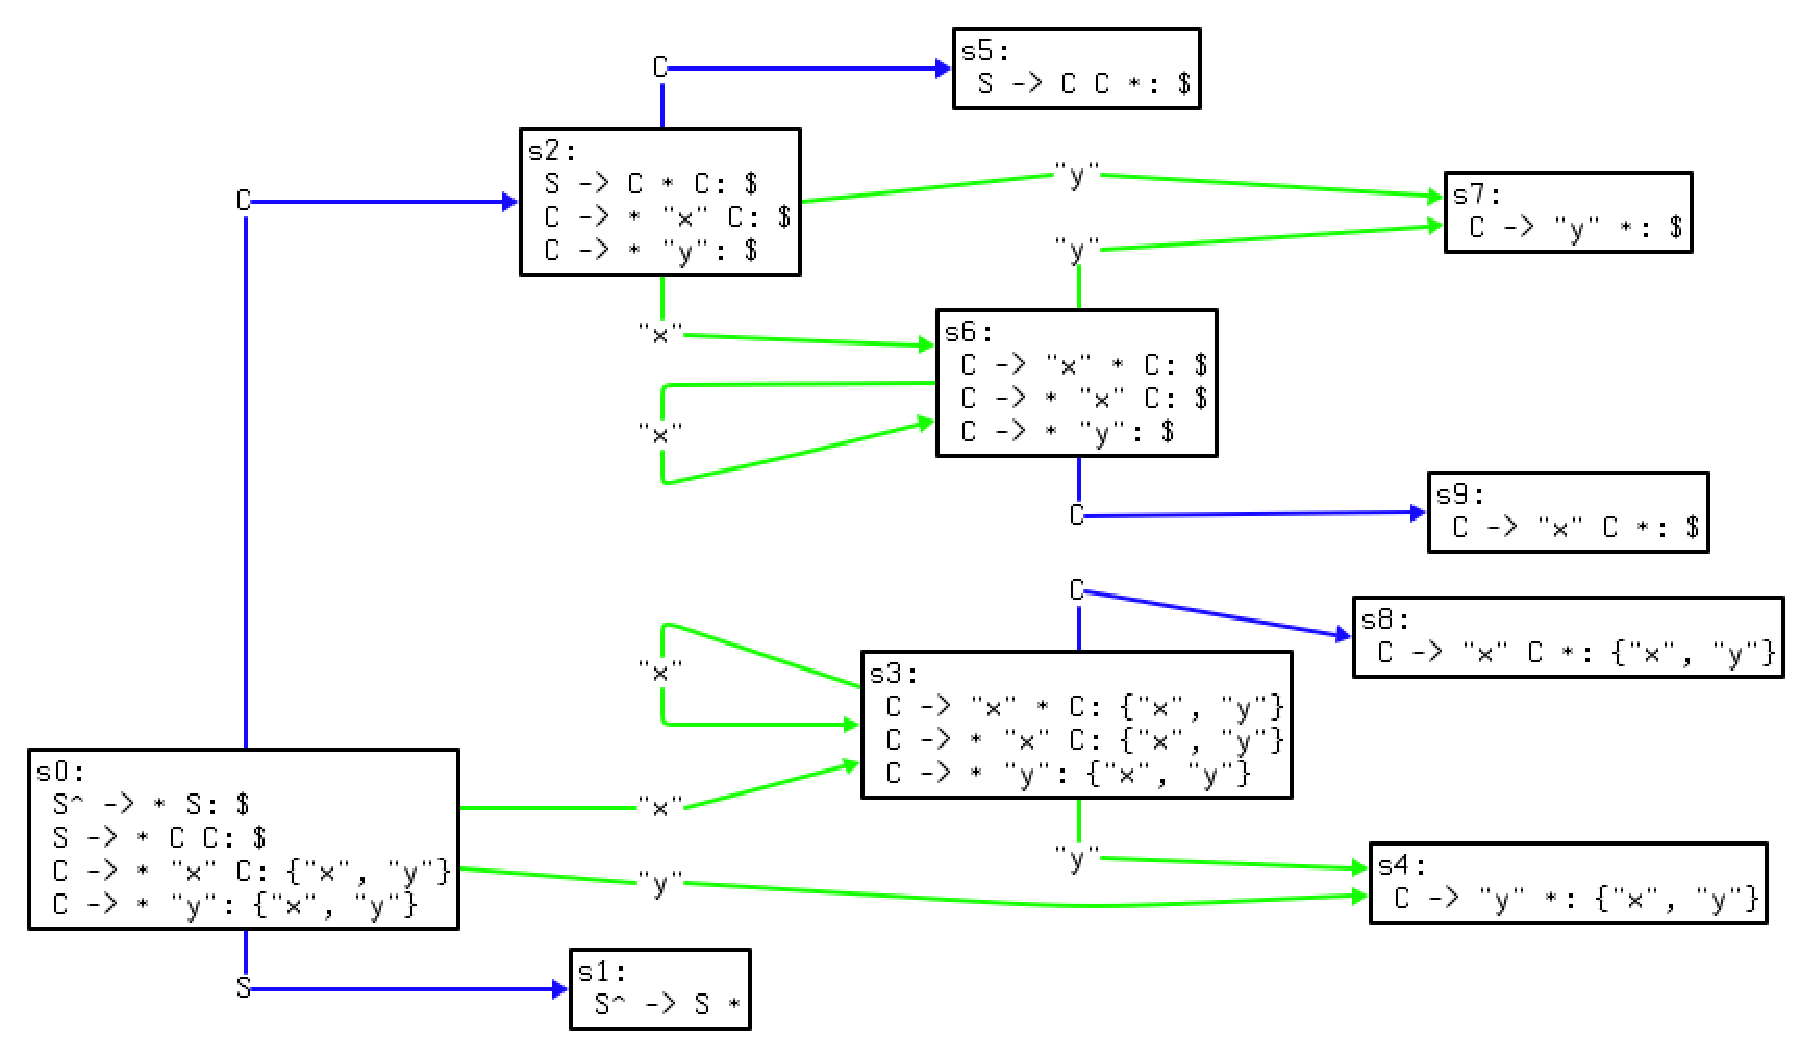
\epsfig{file=Abbildungen/cc-LR.eps, scale=0.5}
      \caption{LR-Goto-Graph f\"ur die Grammatik aus Abbildung \ref{fig:dragon-book.grammar}.}
  \label{fig:cc-LR.eps}
\end{figure}


Abbildung \ref{fig:cc-LR.eps} zeigt den sogenannten \emph{LR-Goto-Graphen} f\"ur diese Grammatik.
Die Knoten dieses Graphen sind die Zust\"ande.  
Betrachten wir den LR-Goto-Graphen, so stellen wir fest, dass die Zust\"ande $s_6$ und
$s_3$ sich nur in den Mengen der Folge-Token unterscheiden, denn es gilt einerseits
\\[0.2cm]
\hspace*{1.3cm}
$s_6 = \Bigl\{ s \rightarrow \squoted{x} \bullet c: \squoted{\symbol{36}}, 
                 c \rightarrow \bullet\, \quoted{x} c:  \squoted{\symbol{36}},
                 c \rightarrow \bullet\, \quoted{y}:    \squoted{\symbol{36}}
       \Bigr\}$, 
\\[0.2cm]
und andererseits haben wir
\\[0.2cm]
\hspace*{1.3cm}
$s_3 = \Bigl\{ s \rightarrow \squoted{x} \bullet c: \{ \squoted{x}, \squoted{y} \}, 
                 c \rightarrow \bullet\, \quoted{x} c:  \{ \squoted{x}, \squoted{y} \},
                 c \rightarrow \bullet\, \quoted{y}:    \{ \squoted{x}, \squoted{y} \}  
       \Bigr\}$.
\\[0.2cm]
Offenbar entsteht die Menge $s_3$ aus der Menge $s_6$ indem \"uberall $\squoted{\symbol{36}}$
durch die Menge $\{ \squoted{x}, \squoted{y}\}$ ersetzt wird.  Genauso kann die Menge $s_7$ in $s_4$
und $s_9$ in $s_8$ \"uberf\"uhrt werden.  Die entscheidende Erkenntnis ist nun, dass die
Funktion $\textsl{goto}()$ unter dieser Art von Transformation invariant ist, denn bei der
Definition dieser Funktion spielt die Menge der Folge-Token keine Rolle.  So sehen wir zum
Beispiel, dass einerseits
\\[0.2cm]
\hspace*{1.3cm}
$\textsl{goto}(s_3, c) = s_8$ \quad und \quad und 
$\textsl{goto}(s_6, c) = s_9$ 
\\[0.2cm]
gilt und dass andererseits der Zustand $s_9$ in den Zustand $s_8$ \"ubergeht, wenn wir
\"uberall in $s_9$ das Terminal $\squoted{\symbol{36}}$ durch die Menge 
 $\{ \squoted{x}, \squoted{y}\}$ ersetzen.  Definieren wir den \emph{Kern}
einer Menge von erweiterten markierten Regeln dadurch, dass wir in jeder Regel die Menge
der Folgetoken wegstreichen, und fassen dann Zust\"ande mit dem selben Kern zusammen, so
erhalten wir den in 
Abbildung \ref{fig:cc-LALR.eps} gezeigten Goto-Graphen.

\begin{figure}[!ht]
\centering
  \hspace*{-0.6cm} 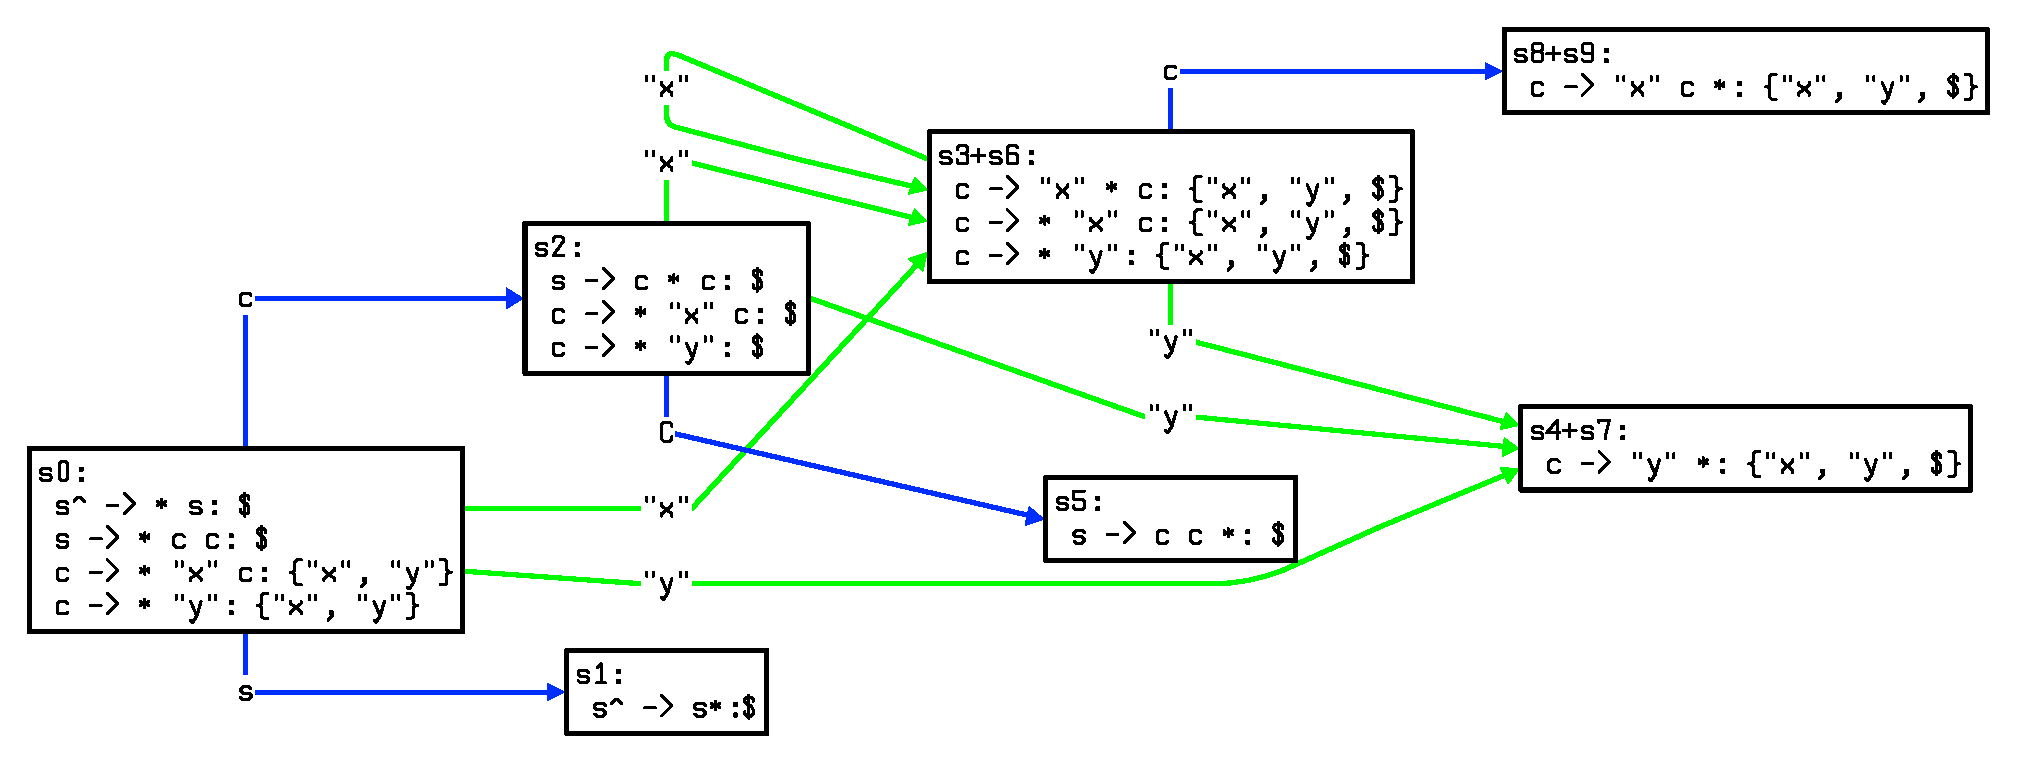
\epsfig{file=Abbildungen/cc-LALR, scale=0.5}
  \caption{Der LALR-Goto-Graph f\"ur die Grammatik aus Abbildung \ref{fig:dragon-book.grammar}.}
  \label{fig:cc-LALR.eps}
\end{figure}

Um die Beobachtungen, die wir bei der Betrachtung der in Abbildung
\ref{fig:dragon-book.grammar} gezeigten Grammatik gemacht gaben, verallgemeinern und formalisieren zu
k\"onnen, definieren wir ein Funktion 
$\textsl{core}()$, die den Kern einer Menge von e.m.R.s berechnet und damit diese Menge in
eine Menge markierter Regeln \"uberf\"uhrt: 
\\[0.2cm]
\hspace*{1.3cm}
$\textsl{core}(\mathcal{M}) := 
   \{ a \rightarrow \beta \bullet \gamma \mid (a \rightarrow \beta \bullet \gamma:L) \in \mathcal{M} \}$. 
\\[0.2cm]
Die Funktion $\textsl{core}()$ entfernt also einfach die Menge der Folge-Tokens von den e.m.R.s.
Wir hatten die Funktion $\textsl{goto}()$ f\"ur eine Menge $\mathcal{M}$ von erweiterten
markierten Regeln und ein Symbol $x$ durch
\\[0.2cm]
\hspace*{1.3cm}
$\textsl{goto}(\mathcal{M}, x) := \textsl{closure}\Bigl( \bigl\{ 
 a \rightarrow \beta\, x \bullet \gamma:L \mid (a \rightarrow \beta \bullet x\, \gamma:L) \in \mathcal{M} 
 \bigr\} \Bigr)
$.
\\[0.2cm]
definiert.  Offenbar spielt die Menge der Folge-Token bei der Berechnung von
$\textsl{goto}(\mathcal{M}, x)$ keine Rolle, formal gilt f\"ur zwei e.m.R.-Mengen
$\mathcal{M}_1$ und $\mathcal{M}_2$ und ein Symbol $x$ die Formel:
\\[0.2cm]
\hspace*{1.3cm}
$\textsl{core}(\mathcal{M}_1) = \textsl{core}(\mathcal{M}_2) \;\Rightarrow\;
 \textsl{core}(\textsl{goto}(\mathcal{M}_1, x)) = 
 \textsl{core}(\textsl{goto}(\mathcal{M}_2, x))
$.
\vspace*{0.2cm}

F\"ur zwei e.m.R.-Mengen $\mathcal{M}$ und $\mathcal{N}$, die
den gleichen Kern haben, definieren wir die \emph{erweiterte Vereinigung}  
$\mathcal{M} \uplus \mathcal{N}$ von $\mathcal{M}$ und $\mathcal{N}$ als
\\[0.2cm]
\hspace*{1.3cm}
$\mathcal{M} \uplus \mathcal{N} := 
   \{ a \rightarrow \beta\bullet \gamma:K \cup L \mid 
      (a \rightarrow \beta\bullet \gamma:K) \in \mathcal{M} \;\wedge\;
      (a \rightarrow \beta\bullet \gamma:L) \in \mathcal{N}
   \}
$.
\\[0.2cm] 
Diese Definition verallgemeinern wir zu einer Operation $\biguplus$, 
die auf einer Menge von Mengen von e.m.R.s definiert ist: Ist $\frak{I}$
eine Menge von Mengen von e.m.R.s, die alle den gleichen Kern haben, gilt also
\[ \frak{I} = \{ \mathcal{M}_1, \cdots, \mathcal{M}_k \} \quad \mbox{mit} \quad
   \textsl{core}(\mathcal{M}_i) = \textsl{core}(\mathcal{M}_j) \quad 
   \mbox{f\"ur alle $i,j\in\{1,\cdots,k\}$,} 
\]
so definieren wir
\[ \biguplus \frak{I} := \mathcal{M}_1 \uplus \cdots \uplus \mathcal{M}_k. 
\]
Es sei nun $\Delta$ die Menge aller Zust\"ande eines LR-Parsers.  Dann ist die Menge der Zust\"ande des
entsprechenden LALR-Parsers durch die erweiterte Vereinigung der Menge aller der Teilmengen 
von $\Delta$ gegeben, deren Elemente den gleichen Kern haben:
\[ \frak{Q} := \left\{ \biguplus \frak{I} \mid \frak{I} \in 2^\Delta \wedge 
      \forall \mathcal{M},\mathcal{N} \in \frak{I}: \textsl{core}(\mathcal{M}) = \textsl{core}(\mathcal{N}) 
      \wedge \mbox{und $\frak{I}$ maximal} 
   \right\}. 
\]
Die Forderung ``$\frak{I}$ maximal'' dr\"uckt in der obigen Definition aus, dass in $\frak{I}$ tats\"achlich
\underline{alle} Mengen aus $\Delta$ zusamengefasst sind, die den selben Kern haben.
Die so definierte Menge $\frak{Q}$ ist die Menge der LALR-Zust\"ande.  

Als n\"achstes \"uberlegen wir, wie sich die Berechnung von $\textsl{goto}(\mathcal{M},X)$
\"andern muss, wenn $\mathcal{M}$ ein Element der Menge $\frak{Q}$ der LALR-Zust\"ande ist.  
Zur Berechnung von $\textsl{goto}(\mathcal{M},X)$ berechnen wir zun\"achst die Menge
\\[0.2cm]
\hspace*{1.3cm}
$\textsl{closure}\Bigl( \bigl\{  
  A \rightarrow \alpha X \bullet \beta:L \mid (A \rightarrow \alpha \bullet X \beta:L) \in \mathcal{M} 
  \bigr\} \Bigr)
$.
\\[0.2cm]
Das Problem ist, dass diese Menge im Allgemeinen kein Element der Menge $\frak{Q}$ ist,
denn die Zust\"ande in $\frak{Q}$ entstehen ja durch die Zusammenfassung mehrerer LR-Zust\"ande.
Die Zust\"ande, die bei der Berechnung von $\frak{Q}$ zusammengefasst werden, haben aber alle den selben
Kern.  Daher enth\"alt die  Menge
\\[0.2cm]
\hspace*{1.3cm}
$\Bigl\{ q \in \frak{Q} \mid \textsl{core}(q) =
  \textsl{core}\bigl(\textsl{closure}\bigl( \bigl\{  
  a \rightarrow \beta\, x \bullet \gamma:L \mid (a \rightarrow \beta \bullet x\, \gamma:L) \in \mathcal{M} 
  \bigr\} \bigr)\bigr)
  \Bigr\}
$
\\[0.2cm]
genau ein Element und dieses Element ist der Wert von $\textsl{goto}(\mathcal{M}, X)$.  Folglich
k\"onnen wir  
\\[0.2cm]
\hspace*{1.3cm}
$\ds\textsl{goto}(\mathcal{M}, X) := \textsl{arb}\Bigl(\Bigl\{ q \in \frak{Q} \mid \textsl{core}(q) =
  \textsl{core}\Bigl(\textsl{closure}\Bigl( \bigl\{  
  a \rightarrow \beta\, X \bullet \gamma:L \mid (a \rightarrow \beta \bullet X\, \gamma:L) \in \mathcal{M} 
  \bigr\} \Bigr)\Bigr)
  \Bigr\} \Bigr)
$
\\[0.2cm]
setzen.  Die hier verwendete Funktion $\textsl{arb}()$ dient dazu, ein beliebiges Element aus einer Menge
zu extrahieren.  Da die Menge, aus der hier das Element extrahiert wird, genau ein Element enth\"alt, ist
$\textsl{goto}(\mathcal{M}, x)$ wohldefiniert.
Die Berechnung des Ausdrucks $\textsl{action}(\mathcal{M}, t)$ \"andert sich gegen\"uber der Berechnung f\"ur
einen LR-Parser nicht. 

\section{Vergleich von SLR-, LR- und LALR-Parsern}
Wir wollen nun die verschiedenen Methoden, mit denen wir in diesem Kapitel
Shift-Reduce-Parser konstruiert haben, vergleichen.  Wir nennen eine Sprache $\mathcal{L}$
eine \emph{SLR-Sprache}, wenn $\mathcal{L}$ von einem SLR-Parser erkannt werden kann.
Die Begriffe \emph{kanonische LR-Sprache} und \emph{LALR-Sprache} werden analog definiert.
 Zwischen diesen Sprachen bestehen die folgende Beziehungen:
\\[0.2cm]
\hspace*{1.3cm}
\emph{SLR-Sprache} $\subsetneq$ \emph{LALR-Sprache} $\subsetneq$ \emph{kanonische LR-Sprache} 
\hspace*{\fill} $(\star)$
\\[0.2cm]
Diese Inklusionen sind leicht zu verstehen:  Bei der Definition der LR-Parser hatten wir
zu den markierten Regeln  Mengen von Folge-Token hinzugef\"ugt.  Dadurch war
es m\"oglich, in bestimmten F\"allen Shift-Reduce- und Reduce-Reduce-Konflikte zu vermeiden.
Da die Zustands-Mengen der kanonischen LR-Parser unter Umst\"anden sehr gro{\ss} werden k\"onnen,
hatten wir dann wieder solche Mengen von erweiterten markierten Regeln zusammengefasst,
f\"ur die die Menge der Folge-Token identisch war.  So hatten wir die LALR-Parser
erhalten.  Durch die Zusammenfassung von Regel-Menge k\"onnen wir
uns allerdings in bestimmten F\"allen Reduce-Reduce-Konflikte einhandeln, so dass die 
Menge der LALR-Sprachen eine Untermenge der kanonischen LR-Sprachen ist.

Wir werden in den folgenden Unterabschnitten zeigen, dass die Inklusionen in $(\star)$ echt sind.  

\subsection{\emph{SLR-Sprache} $\subsetneq$ \emph{LALR-Sprache}}
Die Zust\"ande eines LALR-Parsers enthalten gegen\"uber den Zust\"anden eines SLR-Parsers noch
Mengen von Folge-Token.  Damit sind LALR-Parser mindestens genauso m\"achtig wie SLR-Parser.
Wir zeigen nun, dass LALR-Parser tats\"achlich m\"achtiger als SLR-Parser sind.  Um diese
Behauptung zu belegen, pr\"asentieren wir eine Grammatik, f\"ur die es zwar einen LALR-Parser,
aber keinen SLR-Parser gibt.  Wir hatten auf Seite \pageref{fig:reduce-reduce-conflict.grammar}
gesehen, dass die Grammatik
\\[0.2cm]
\hspace*{1.3cm}
$s \;\rightarrow\; a \quoted{x} a \quoted{y} \mid b \quoted{y} b \quoted{x}$, \quad
$a \;\rightarrow\;\varepsilon$, \quad
$b \;\rightarrow\; \varepsilon$
\\[0.2cm]
keine SLR-Grammatik ist.  Sp\"ater hatten wir gesehen, dass diese Grammatik von einem
kanonischen LR-Parser geparst werden kann.  Wir zeigen nun, dass diese Grammatik auch von
einem LALR-Parser geparst werden kann.  Dazu berechnen wir die Menge der LALR-Zust\"ande.
Dazu ist zun\"achst die Menge der kanonischen LR-Zust\"ande zu berechnen.  Diese Berechnung
hatten wir bereits fr\"uher durchgef\"uhrt und dabei die folgenden Zust\"ande erhalten:
\begin{enumerate}
\item $s_0  = \bigl\{ \widehat{s} \rightarrow \bullet\, s:\symbol{36},
                     s \rightarrow \bullet\, a \squoted{x} a \squoted{y}:\symbol{36},
                     s \rightarrow \bullet\, b \squoted{y} b \squoted{x}:\symbol{36},
                     a \rightarrow \bullet\,: \squoted{x},
                     b \rightarrow \bullet\,: \squoted{y}
              \bigr\}
      $,
\item $s_1 = \bigl\{ s \rightarrow a \bullet \squoted{x} a \squoted{y}:\symbol{36} \bigr\}$,
\item $s_2 = \bigl\{ \widehat{s} \rightarrow s \bullet:\symbol{36} \bigr\}$,
\item $s_3 = \bigl\{ s \rightarrow b \bullet \squoted{y} b \squoted{x}: \symbol{36} \bigr\}$,
\item $s_4 = \bigl\{ s \rightarrow b \squoted{y} \bullet b \squoted{x}: \symbol{36},
                     b \rightarrow \bullet\,: \squoted{x}
             \bigr\}
      $,
\item $s_5 = \bigl\{ s \rightarrow b \squoted{y} b \bullet \squoted{x}: \symbol{36} \bigr\}$,
\item $s_6 = \bigl\{ s \rightarrow b \squoted{y} b \squoted{x} \bullet: \symbol{36} \bigr\}$,
\item $s_7 = \bigl\{ s \rightarrow a \squoted{x} \bullet a \squoted{y}:\symbol{36},
                     a \rightarrow \bullet\,: \squoted{y}
              \bigr\}
      $,
\item $s_8 = \bigl\{ s \rightarrow a \squoted{x} a \bullet \squoted{y}:\symbol{36} \bigr\}$,
\item $s_9 = \bigl\{ s \rightarrow a \squoted{x} a \squoted{y} \bullet :\symbol{36} \bigr\}$.
\end{enumerate}
Wir stellen fest, dass die Kerne aller hier aufgelisteten Zust\"ande verschieden sind.
Damit stimmt bei dieser Grammatik die Menge der Zust\"ande des LALR-Parser mit der Menge der
Zust\"ande des kanonischen LR-Parsers \"uberein.  Daraus folgt, dass es auch bei
den LALR-Zust\"anden keine Konflikte gibt, denn beim \"Ubergang von kanonischen LR-Parsern zu
LALR-Parsern haben wir lediglich Zust\"ande mit gleichem Kern zusammengefasst, die
Definition der Funktionen $\textsl{goto}()$ und $\textsl{action}()$ blieb unver\"andert.

\subsection{\emph{LALR-Sprache} $\subsetneq$ \emph{kanonische LR-Sprache}}
Wir hatten LALR-Parser dadurch definiert, dass wir verschiedene Zust\"ande eines kanonischen LR-Parsers
zusammengefasst haben.  Damit ist klar, dass kanonische LR-Parser mindestens so m\"achtig
sind wie LALR-Parser.  Um zu zeigen, dass kanonische LR-Parser tats\"achlich m\"achtiger sind
als LALR-Parser, ben\"otigen wir eine Grammatik, f\"ur die sich zwar ein kanonischer LR-Parser,
aber kein LALR-Parser erzeugen l\"asst.  Abbildung \ref{fig:lr-but-notlalr.g} zeigt eine
solche Grammatik, die ich dem Drachenbuch entnommen habe.

\begin{figure}[htbp]
  \begin{center}    
  \framebox{
  \framebox{
  \begin{minipage}[t]{5.5cm}
    \vspace*{-0.3cm}

  \begin{eqnarray*}
  s  & \rightarrow & \quoted{v} a \quoted{y} \\
     & \mid        & \quoted{w} b \quoted{y} \\
     & \mid        & \quoted{v} b \quoted{z} \\
     & \mid        & \quoted{w} a \quoted{z} \\[0.1cm]
  a  & \rightarrow & \quoted{x}              \\[0.1cm]
  b  & \rightarrow & \quoted{x}              
  \end{eqnarray*}
  \vspace*{-0.5cm}

  \end{minipage}}}
  \vspace*{-0.3cm}

  \end{center}
  \caption{Eine kanonische LR-Grammatik, die keine LALR-Grammatik ist.}
  \label{fig:lr-but-notlalr.g}
\end{figure}

Wir berechnen zun\"achst die Menge der Zust\"ande eines kanonischen LR-Parsers f\"ur diese
Grammatik.  Wir erhalten dabei die folgende Mengen von erweiterten markierten Regeln:
\begin{enumerate}
\item $s_0 = \textsl{closure}(\widehat{s} \rightarrow \bullet\, \;s: \symbol{36}) =
       \{
       \begin{array}[t]{lcl}
         \widehat{s} & \rightarrow & \bullet \;s: \symbol{36},                \\
         s           & \rightarrow & \bullet \squoted{v} a \squoted{y}: \symbol{36}, \\
         s           & \rightarrow & \bullet \squoted{v} b \squoted{z}: \symbol{36}, \\
         s           & \rightarrow & \bullet \squoted{w} a \squoted{z}: \symbol{36}, \\
         s           & \rightarrow & \bullet \squoted{w} b \squoted{y}: \symbol{36}\;\},
        \end{array}
       $
\item $s_1 = \textsl{goto}(s_0, s) =\{ \widehat{s} \rightarrow s \bullet: \symbol{36} \}$
\item $s_2 = \textsl{goto}(s_0, \quoted{v}) = \{ 
       \begin{array}[t]{lcl}
        s & \rightarrow & \squoted{v} \bullet b \squoted{z}: \symbol{36}, \\
        s & \rightarrow & \squoted{v} \bullet a \squoted{y}: \symbol{36}, \\
        a & \rightarrow & \bullet \squoted{x}: \squoted{y}, \\
        b & \rightarrow & \bullet \squoted{x}: \squoted{z}\; \},
       \end{array}
      $
\item $s_3 = \textsl{goto}(s_0, \quoted{w}) = \{ 
       \begin{array}[t]{lcl}
       s & \rightarrow & \squoted{w} \bullet a \squoted{z}: \symbol{36},  \\
       s & \rightarrow & \squoted{w} \bullet b \squoted{y}: \symbol{36},  \\
       a & \rightarrow & \bullet \squoted{x}: \squoted{z},                \\
       b & \rightarrow & \bullet \squoted{x}: \squoted{y}\; \},
       \end{array}
      $
\item $s_4 = \textsl{goto}(s_2, \quoted{x}) =
             \{ a \rightarrow \squoted{x} \bullet: \squoted{y},\;
                b \rightarrow \squoted{x} \bullet: \squoted{z} \}$,
\item $s_5 = \textsl{goto}(s_3, \quoted{x}) =
             \{ a \rightarrow \squoted{x} \bullet: \squoted{z},\,
                b \rightarrow \squoted{x} \bullet: \squoted{y} \}$,
\item $s_6 = \textsl{goto}(s_2, a) =
             \{ s \rightarrow \squoted{v} a \bullet \squoted{y}: \symbol{36} \}$,
\item $s_7 = \textsl{goto}(s_6, \quoted{y}) =
             \{ s \rightarrow \squoted{v} a \squoted{y} \bullet: \symbol{36} \}$,
\item $s_8 = \textsl{goto}(s_2, b) =
             \{ s \rightarrow \squoted{v} b \bullet \squoted{z}: \symbol{36} \}$,
\item $s_9 = \textsl{goto}(s_8, \quoted{z}) =
             \{ s \rightarrow \squoted{v} b \squoted{z} \bullet: \symbol{36} \}$,
\item $s_{10} = \textsl{goto}(s_3, a) =
                \{ s \rightarrow \squoted{w} a \bullet \squoted{z}: \symbol{36} \}$,
\item $s_{11} = \textsl{goto}(s_{10}, \quoted{z}) =
                \{ s \rightarrow \squoted{w} a \squoted{z} \bullet: \symbol{36} \}$,
\item $s_{12} = \textsl{goto}(s_3, b) =
                \{ s \rightarrow \squoted{w} b \bullet \squoted{y}: \symbol{36} \}$,
\item $s_{13} = \textsl{goto}(s_{12}, \quoted{y}) =
                \{ s \rightarrow \squoted{w} b \squoted{y} \bullet: \symbol{36} \}$.
\end{enumerate}
Die einzigen Zust\"ande, bei denen es Konflikte geben k\"onnte, sind die Mengen $s_4$ und
$s_5$, denn hier sind prinzipiell sowohl Reduktionen mit der Regel
\\[0.2cm]
\hspace*{1.3cm}
$a \rightarrow \squoted{x}$ \quad als auch mit \quad
$b \rightarrow \squoted{x}$
\\[0.2cm]
m\"oglich.  Da allerdings die Mengen der Folge-Token einen leeren Durchschnitt haben, gibt
es tats\"achlich keinen Konflikt und die Grammatik ist eine kanonische LR-Grammatik.

Wir berechnen als n\"achstes die LALR-Zust\"ande der oben angegebenen Grammatik.  Die einzigen
Zust\"ande, die einen gemeinsamen Kern haben, sind die beiden Zust\"ande $s_4$ und $s_5$, denn
es gilt
\\[0.2cm]
\hspace*{1.3cm}
$\textsl{core}(s_4) = \{ a \rightarrow \squoted{x} \bullet,\;
                b \rightarrow \squoted{x} \bullet \} = \textsl{core}(s_5)$.
\\[0.2cm]
Bei der Berechnung der LALR-Zust\"ande werden diese beiden Zust\"ande zu einem Zustand
$s_{\{4,5\}}$ zusammengefasst.  Dieser neue Zustand hat die Form
\\[0.2cm]
\hspace*{1.3cm}
$s_{\{4,5\}} = \bigl\{ A \rightarrow \squoted{x} \bullet: \{\squoted{y}, \squoted{z} \},\;
                       B \rightarrow \squoted{x} \bullet: \{\squoted{y}, \squoted{z} \} \bigr\}$.
\\[0.2cm]
Hier gibt es offensichtlich  einen Reduce-Reduce-Konflikt, denn einerseits haben wir
\\[0.2cm]
\hspace*{1.3cm}
$\textsl{action}(s_{\{4,5\}}, \squoted{y}) = \pair(\textsl{reduce}, A \rightarrow \squoted{x})$,
\\[0.2cm]
andererseits gilt aber auch
\\[0.2cm]
\hspace*{1.3cm}
$\textsl{action}(s_{\{4,5\}}, \squoted{y}) = \pair(\textsl{reduce}, B \rightarrow \squoted{x})$.

\exercise
Es sei $G = \langle V, T, R, s \rangle$ eine LR-Grammatik und $\mathcal{N}$ sei die Menge der
LALR-Zust\"ande der Grammatik.  \"Uberlegen Sie, warum es in der Menge $\mathcal{N}$ keine
Shift-Reduce-Konflikte geben kann.  \eox


\paragraph{Historical Notes}
The theory of LALR parsing is due to Franklin L.~DeRemer \cite{deRemer:71}.  At the time of its
invention,  the space savings of LALR parsing in comparison to LR parsing were crucial.  


\subsection{Bewertung der verschiedenen Methoden}
F\"ur die Praxis sind SLR-Parser nicht ausreichend, denn es gibt eine Reihe praktisch
relevanter Sprach-Konstrukte, f\"ur die sich kein SLR-Parser erzeugen l\"asst.  Kanonische
LR-Parser sind wesentlich m\"achtiger, ben\"otigen allerdings oft deutlich mehr Zust\"ande. 
Hier stellen LALR-Parser einen Kompromiss dar:  Einerseits sind LALR-Sprachen fast so
ausdrucksstark  wie kanonische LR-Sprachen, andererseits liegt der Speicherbedarf von
LALR-Parsern in der gleichen Gr\"o{\ss}enordnung wie der Speicherbedarf von SLR-Parsern.  Beispielsweise
hat die SLR-Parse-Tabelle f\"ur die Sprache \texttt{C} insgesamt 349 Zust\"ande, die entsprechende
LR-Parse-Tabelle kommt auf 1572 Zust\"ande, w\"ahrend der LALR-Parser mit 350 Zust\"anden auskommt und damit nur
einen Zustand mehr als der SLR-Parser hat.  
In den heute in der Regel zur Verf\"ugung stehenden Hauptspeichern lassen sich allerdings
auch kanonische LR-Parser meist m\"uhelos unterbringen, so dass es eigentlich keinen zwingenden
Grund mehr gibt, statt eines LR-Parsers einen LALR-Parser einzusetzen.  

Andererseits wird niemand einen LALR-Parser oder einen kanonischen LR-Parser von Hand
programmieren wollen.  Statt dessen werden Sie sp\"ater einen Parser-Generator wie \textsl{Bison}
oder \textsl{JavaCup} einsetzen, der Ihnen einen  Parser generiert.  Das Werkzeug Bison
ist ein Parser-Generator f\"ur \texttt{C}, \texttt{C++} und bietet auch eine, allerdings leider noch
experimentelle, Unterst\"utzung f\"ur \textsl{Java},
w\"ahrend \textsl{JavaCup} auf die Sprache \textsl{Java} beschr\"ankt ist.  Falls Sie
\textsl{JavaCup} benutzen, haben Sie keine Wahl, denn dieses Werkzeug erzeugt immer einen
LALR-Parser.  Bei \href{http://www.gnu.org/software/bison/manual/bison.html}{\textsl{Bison}} ist es
ab der Version 3.0  auch m\"oglich, einen LR-Parser zu erzeugen.



%%% Local Variables: 
%%% mode: latex
%%% TeX-master: "formal-languages"
%%% End: 
